\documentclass[12 pt]{report}

\pagenumbering{arabic}

%\usepackage{caption}
\usepackage[nottoc]{tocbibind}
\usepackage{hyperref}
\usepackage[a4paper,top=2cm,left=3cm,right=3cm,bottom=2cm]{geometry}
\usepackage{graphicx}
\usepackage{amsmath,amssymb}
\newcommand{\tarc}{\mbox{\large$\frown$}}
\newcommand{\arc}[1]{\stackrel{\tarc}{#1}}
\usepackage{inputenc}
\usepackage{hyperref}
%\pagestyle{empty}

\graphicspath{./}
\usepackage{float}
\usepackage{setspace}

\linespread{1.3}
\usepackage{multirow}
\usepackage{amsfonts}
\usepackage[export]{adjustbox}

\usepackage{xcolor}
\usepackage{hyperref}


\usepackage{mathtools}
\DeclarePairedDelimiter{\ceil}{\lceil}{\rceil}

\usepackage{enumerate}

\hypersetup{colorlinks=true,linkcolor=black,urlcolor=blue}


\usepackage{xepersian}

\settextfont[]{B Yas}
%\settextfont[]{B Nazanin}
\setdigitfont{B Yas}
\pagestyle{empty}

\begin{document}
	\begin{titlepage}

	\begin{center}
		
		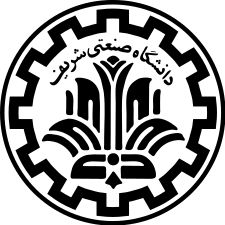
\includegraphics[width=2cm]{images/tuoslogo.png}
		\\
		{ دانشگاه صنعتی شریف  }
		\\[6cm]
		\linespread{1.5}{\huge { \lr{\textit{Skein Hashing}} }}
		
		پروژه مستندسازی پیاده‌سازی سخت افزاری الگوریتم به زبان 
		 \lr{\textit{Verilog}}
		\\[4cm]
		\linespread{1}
		
		{\Large گروه 4 }
		\\[0.4cm]
		{\small سید پارسا اسکندر
			\\[0.2cm] کیمیا یزدانی
			\\[0.2cm] الهه خدایی 
			\\[0.2cm] وحید زهتاب 
			\\[0.2cm] آروین آذرمینا
			\\[0.5cm]
		}
	
		{\large
			\emph{استاد: }
			فرشاد بهاروند
		}
		\\[4cm]
		
		
		{\large بهار ۹۸ }
	\end{center}
	
\end{titlepage}
	\pagebreak
	\chapter*{
چکیده‌ی مقاله
}
\pagestyle{empty}

در این مقاله که در مورد یکی از روش‌های \lr{hash}  به نام \lr{Skein} توضیح داده خواهد شد. و هم‌چنین توضیح و مستند برنامه‌های داده شده به دو زبان \lr{C } به عنوان مدل طلایی و \lr{verilog} به عنوان طرح سخت‌افزاری , آورده خواهد شد .
در انتها نیز تفاوت‌های این دو مدل و دلایل اختلاف آن‌ها (‌ نقاط اشتباه آن‌ها در پیاده‌سازی) تحلیل خواهد شد.
	\tableofcontents
	\chapter{معرفی الگوریتم
\lr{Skein}
}
\section{
مقدمه
}
دردنیای امروز، با افزایش لحظه‌ای اطلاعات در جهان، روز‌ به ‌روز رمزنگاری و رمزگذاری اطلاعات اهمیت دوچندانی پیدا می‌کند.برای مثال برقراری امنیت سیستم‌ها و شبکه‌های رایانه‌ای، ذخیره‌ی اطلاعات مهم و حساس و ... همگی مثال‌هایی هستند که بدون رمزنگاری و رمزگذاری ممکن نخواهند بود. بدون اغراق، بدون رمزگذاری و رمزنگاری، اینترنت به شکلی که امروز وجود دارد به هیچ عنوان وجود نمی‌داشت.
راه‌های بسیار متفاوتی برای رمزنگاری و رمزگذاری وجود دارد، یکی از مهم‌ترینِ آنها، استفاده از توابع رمزگذاریِ بر پایه ی
\textit{ 
	درهم‌سازی (
\lr{Hashing}
)
}
می باشد. درهم‌سازی به خودی خود پرکاربرد ترین داده‌ساختار استفاده شده در علوم رایانه‌ای است. برخی از توابع درهم‌سازی شامل ویژگی‌هایی هستند که آنهارا برای استفاده برای کاربرد‌هایی چون رمزنگاری بسیار مناسب می‌کند. مهم‌ترین و پرکاربردترین این توابع، توابعی از خانواده‌ی 
\textit{\lr{SHA}}
یا 
\textit{\lr{Secure Hashing Algorithms}}
می‌باشند، توابعی چون 
\lr{MD-5}
،
\lr{SHA-0}
،
\lr{SHA-1}
،
\lr{SHA-2}
و 
\lr{SHA-3}
که هر کدام خود شامل خانواده ای از توابع مخصوص کاربرد‌های خاص خود هستند.

توابع خانواده ی 
\lr{SHA}
توسط گروهی به نام 
\textit{\lr{NIST}}
که کوتاه شده‌ی عبارت
\textit{\lr{National Institute of Standards and Technology}}
است، برگزیده می‌شوند. برای انتخاب هریک از ورژن های توابع این خانواده، ابتدا توابعی پیشنهاد شده، پس از آن تعدادی از آنها به عنوان فینالیست توسط 
\lr{NIST}
اعلام شده و در نهایت از بین فینالیست‌ها، یک تابع به عنوان ورژن جدید از توابع 
\lr{SHA}
معرفی می‌شود.

	تابع مورد بررسی در این مقاله یکی از توابع فینالیست برای انتخاب 
	\lr{SHA-3}
	می‌باشد که 
	\lr{Skein}
	نام دارد. 
	
\section{
معرفی اجمالی الگوریتم
}
الگوریتم 
\textit{ \lr{Skein}}
  یکی از خانواده های توابع درهم سازی است که  بر‌اساس اندازه‌ی بلاک‌های داخلی سه نوع مختلف ۲۵۶ ، ۵۱۲  و ۱۰۲۴ بیتی دارد  .
  الگوریتم مورد بررسی در این مقاله مربوط به اندازه‌ی داخلی ۵۱۲ بیتی آن یعنی
  \lr{skein512}
  می‌باشد. در بین این سه نوع کلی از توابع
  \lr{skein}
  ،
 \lr{skein512}
 به عنوان تابع اصلی به کار می‌رود اما لازم به ذکر است که سرعت 
 \lr{skein1024}
دو برابر
 \lr{skein512}
 می‌باشد و 
  \lr{skein256}
 زمانی به کار می رود که نیازمند حجم کمی از رم  (حدود ۱۰۰ بایت) باشد .
 
  درحالت کلی توابع
    \lr{skein}
   توانایی درهم‌سازی ورودی به هر اندازه اندازه‌ای را دارد اما اندازه‌ی خروجی آن، معمولا یکی از حالت های ۲۵۶ یا ۵۱۲ یا ۱۰۲۴ بیتی است. 
  

\pagebreak
\section{
روند اجرایی الگوریتم
}
ایده ی اصلی توابع \lr{Skein}  استفاده از
\textit{ \lr{Tweakable Block Ciphers}}
  یا بلاک های رمزگذاری قابل تنظیم است .
همه‌ی توابع 
\lr{skein}
از سه بخش کلی تشکیل شده اند:
\begin{itemize}
	\item 
	\lr{\textit{\textbf{Threefish}}} 
	یا بلاک های رمزنگاری قابل تنظیم
	\item
	\lr{
		\textit{
			\textbf{Unique Block Iteration (UBI)}
		}
	}

	\item
	\textbf{\lr{\textit{\textbf{Optional Argument System}}} } 
	
\end{itemize}
این سه بخش در کنار هم توابع درهم‌سازی
\lr{skein}
را تشکیل می‌دهند.
 در ادامه به تفصیل به عملکرد هریک از این بخش ها خواهیم‌ پرداخت.
 
\subsection{
	عملکرد
	\lr{Threefish}
}
در‌الگوریتم های 
 \lr{skein}
 بسته به نوع تابع درهم‌سازی از بلاک‌های رمزگذاری استفاده می‌شود که به صورت زنجیره‌ای به یکدیگر متصل شده‌اند، اندازه‌ی این بلاک‌ها بسته به نوع الگوریتم 
 ۲۵۶، ۵۱۲ یا ۱۰۲۴ بیت یا درواقع ۴، ۸ یا ۱۶ بسته‌ی ۶۴ بیتی از داده ها ‌می‌باشد. بلاک های رمزنگاری هرکدام از ترکیب دو تابع غیر خطی به نام های درهم‌سازی
 (
\textit{ \lr{Mix}}
 )
 و جابه‌جایی (
 \textit{ \lr{Permutation}}
)
تشکیل شده‌اند، هر بلاک رمزگذاری با بلاک‌های رمزگذاری دیگر سری شده و زنجیره ای از بلاک‌های رمزگذاری را تشکیل می‌دهند. علاوه براین بلاک‌ها، میان هر ۴ بلاک متوالی به مقادیر محاسبه شده تا آنجا مقادیر کلید هایی مربوط با آن دوره، افزوده می‌شود که به آنها 
\textit{\lr{Subkey}}
گفته‌میشود. در تصویر زیر شمایی کلی از فرایند توضیح داده‌شده قابل مشاهده است:
\begin{figure}[H]
	\centering
	\includegraphics[width=7cm]{Images/Introduction/cipherblock_dataflow.png}	
	\caption{
		شمای کلی از کارکرد بلاک‌های رمزگذاری قابل تنظیم 
	}
\end{figure}
درادامه به توضیح هر‌یک از این توابع می‌پردازیم.
\pagebreak

\subsubsection{
تابع درهم‌سازی (
\lr{Mix}
)
}
این تابع غیر خطی دو بسته‌ی ۶۴ بیتی از داده‌ها ‌را به عنوان ورودی دریافت کرده و دو بسته‌ی ۶۴ بیتی دیگر که حاصلی از ترکیب دو بسته‌ی ورودی هستند را در خروجی تحویل می‌دهد.اگر بسته های ورودی به این تابع به ترتیب ارزش، 
$x_0$ 
و
$x_1$
باشند، بسته‌های خروجی این تابع از فورمول‌های زیر به دست می‌‌آیند:
$$y_0 = x_0 + x_1$$
$$y_1 = (x_0 + x_1) \oplus ( x_1 \lll R_{(d\ mod\  8),j})$$
و از لحاظ ساختار کلی، شمای حرکت داده در این تابع به شکل زیر خواهد بود:


\begin{figure}[H]
	\centering
	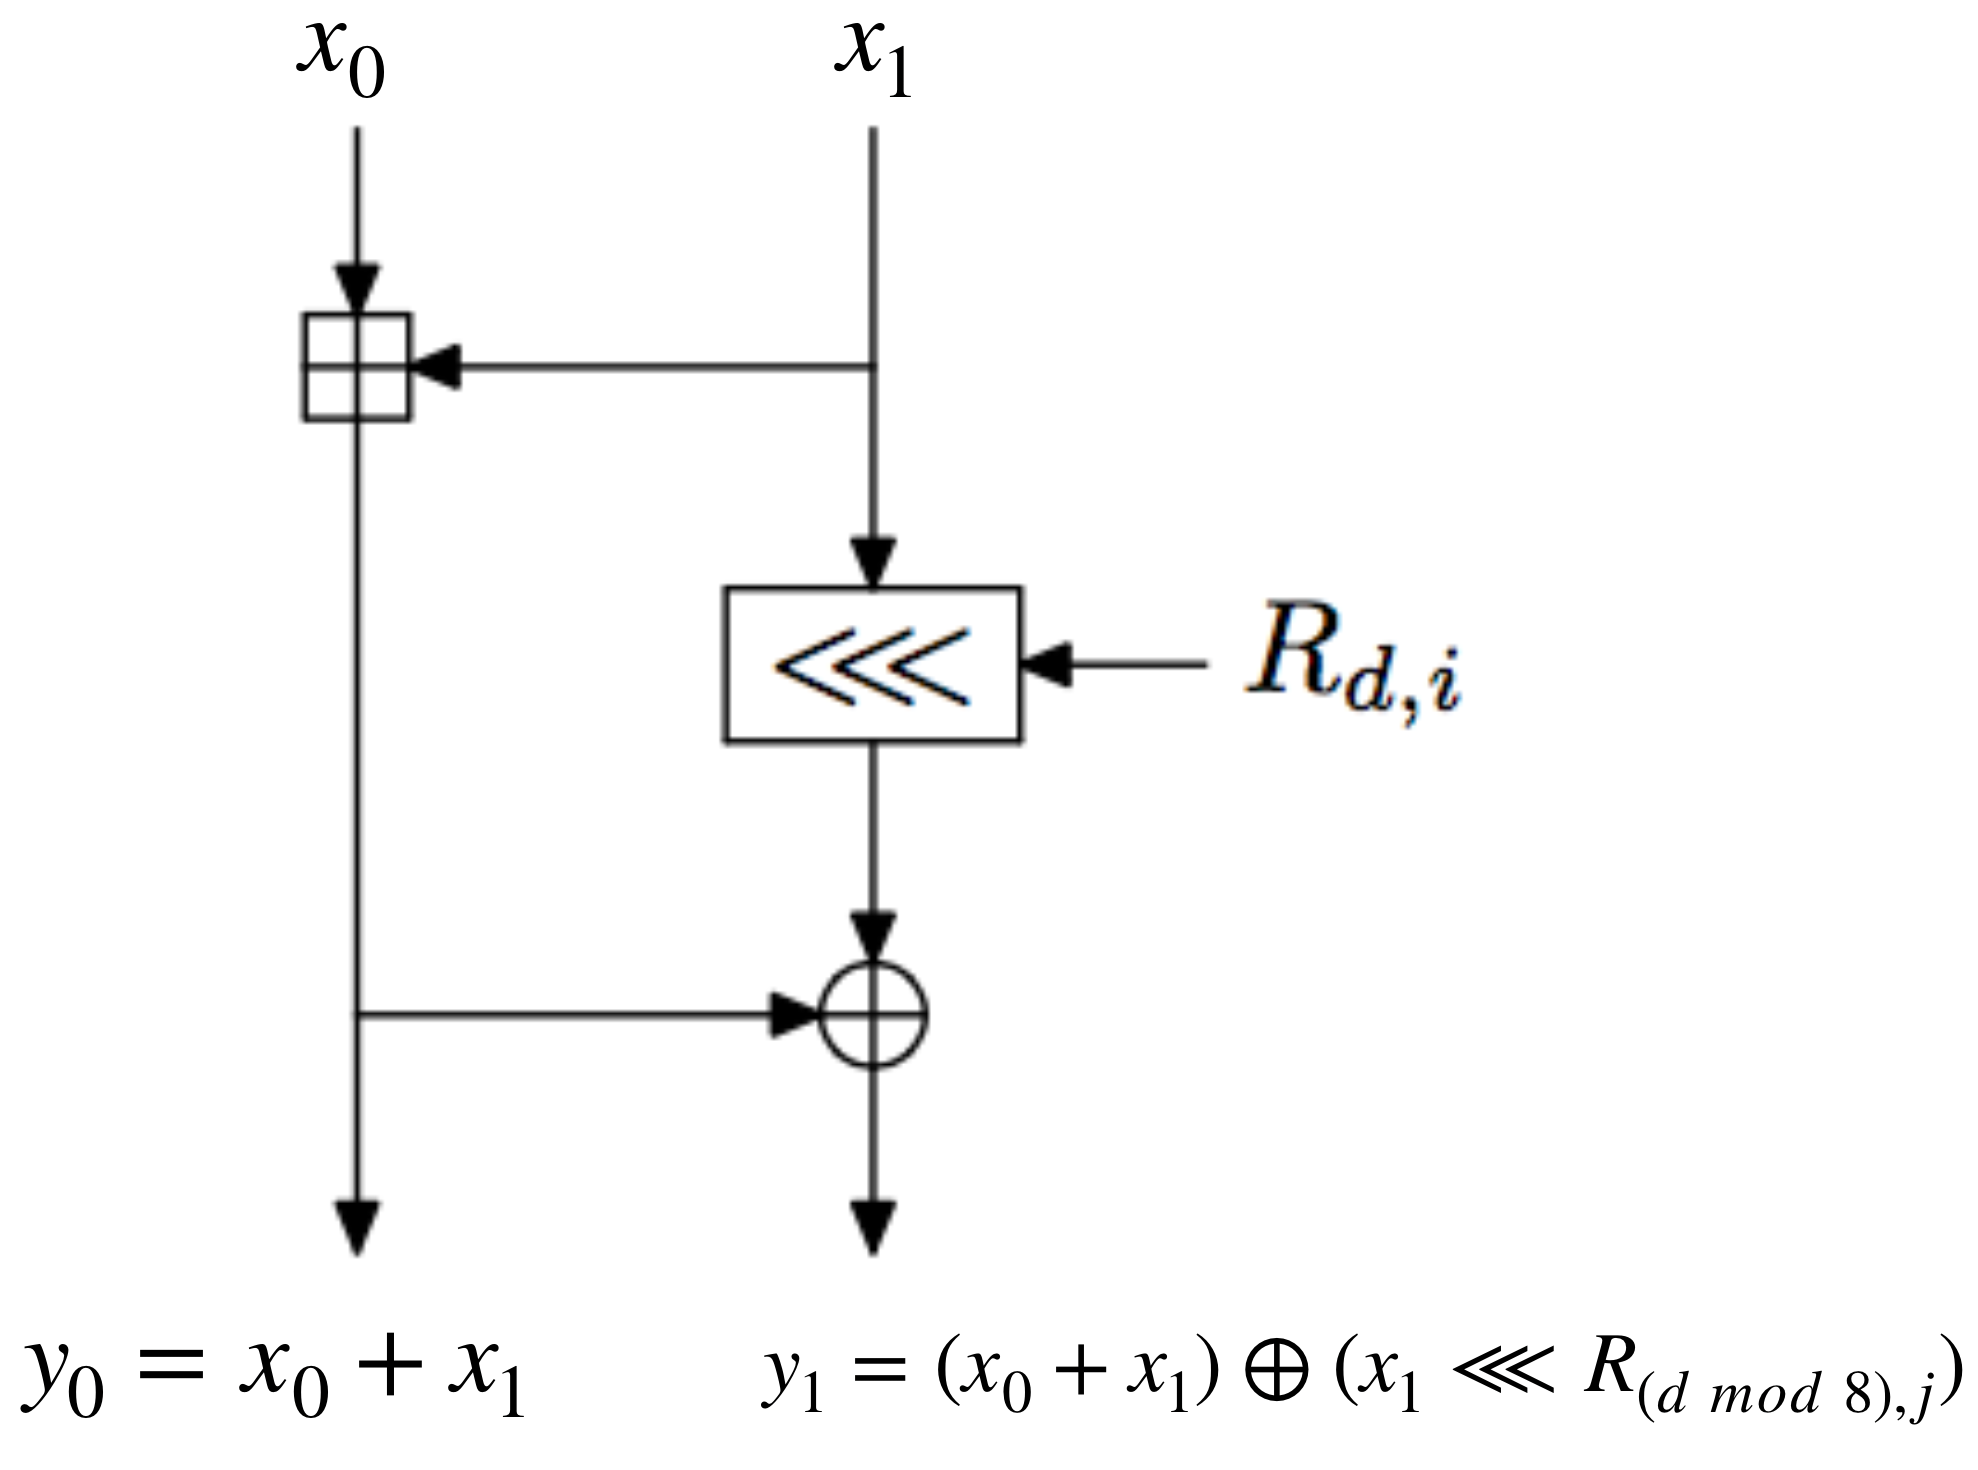
\includegraphics[width=7cm]{Images/Introduction/mix_function_dataflow.png}	
	\caption{
		شمای کلی از کارکرد تابع درهم‌سازی (\lr{Mix})
	}
\end{figure}


عدد
$d$
 شمارنده‌ی بلاک‌های رمزگذاری‌ می باشد که از صفر شروع شده است و عدد $j$ معرف شمارنده‌ی توابع درهم‌سازی (\lr{Mix}) داخل هر بلاک رمزگذاری است به صورتی که  عدد $j$  مربوط به تابعی که پرارزش‌ترین بسته‌های ورودی را دریافت می کند صفر و عدد $j$ مربوط به تابعی که کم‌ارزش‌ترین بسته‌ها را به عنوان ورودی دریافت می‌کند برابر 
$N_W/2 - 1$ 
‌باشد، که در آن 
$N_W$
تعداد بسته‌های موجود در بلاک‌های رمزگذاری است.


عدد 
$ R_{(d\ mod\  8),j}$
تعداد چرخش به چپ‌های لازم برای بسته‌ی ورودی دوم در تابع درهم‌سازی (\lr{Mix}) $j$ ام در بلاک رمزگذاری $d$ ام را مشخص می کند که مقدار آن  به ازای مقادیر مختلفی از 
$j$ و
$d$ و
$N_W$ 
در جدول زیر قابل مشاهده است:
  
  \begin{figure}[H]
  	\centering
  	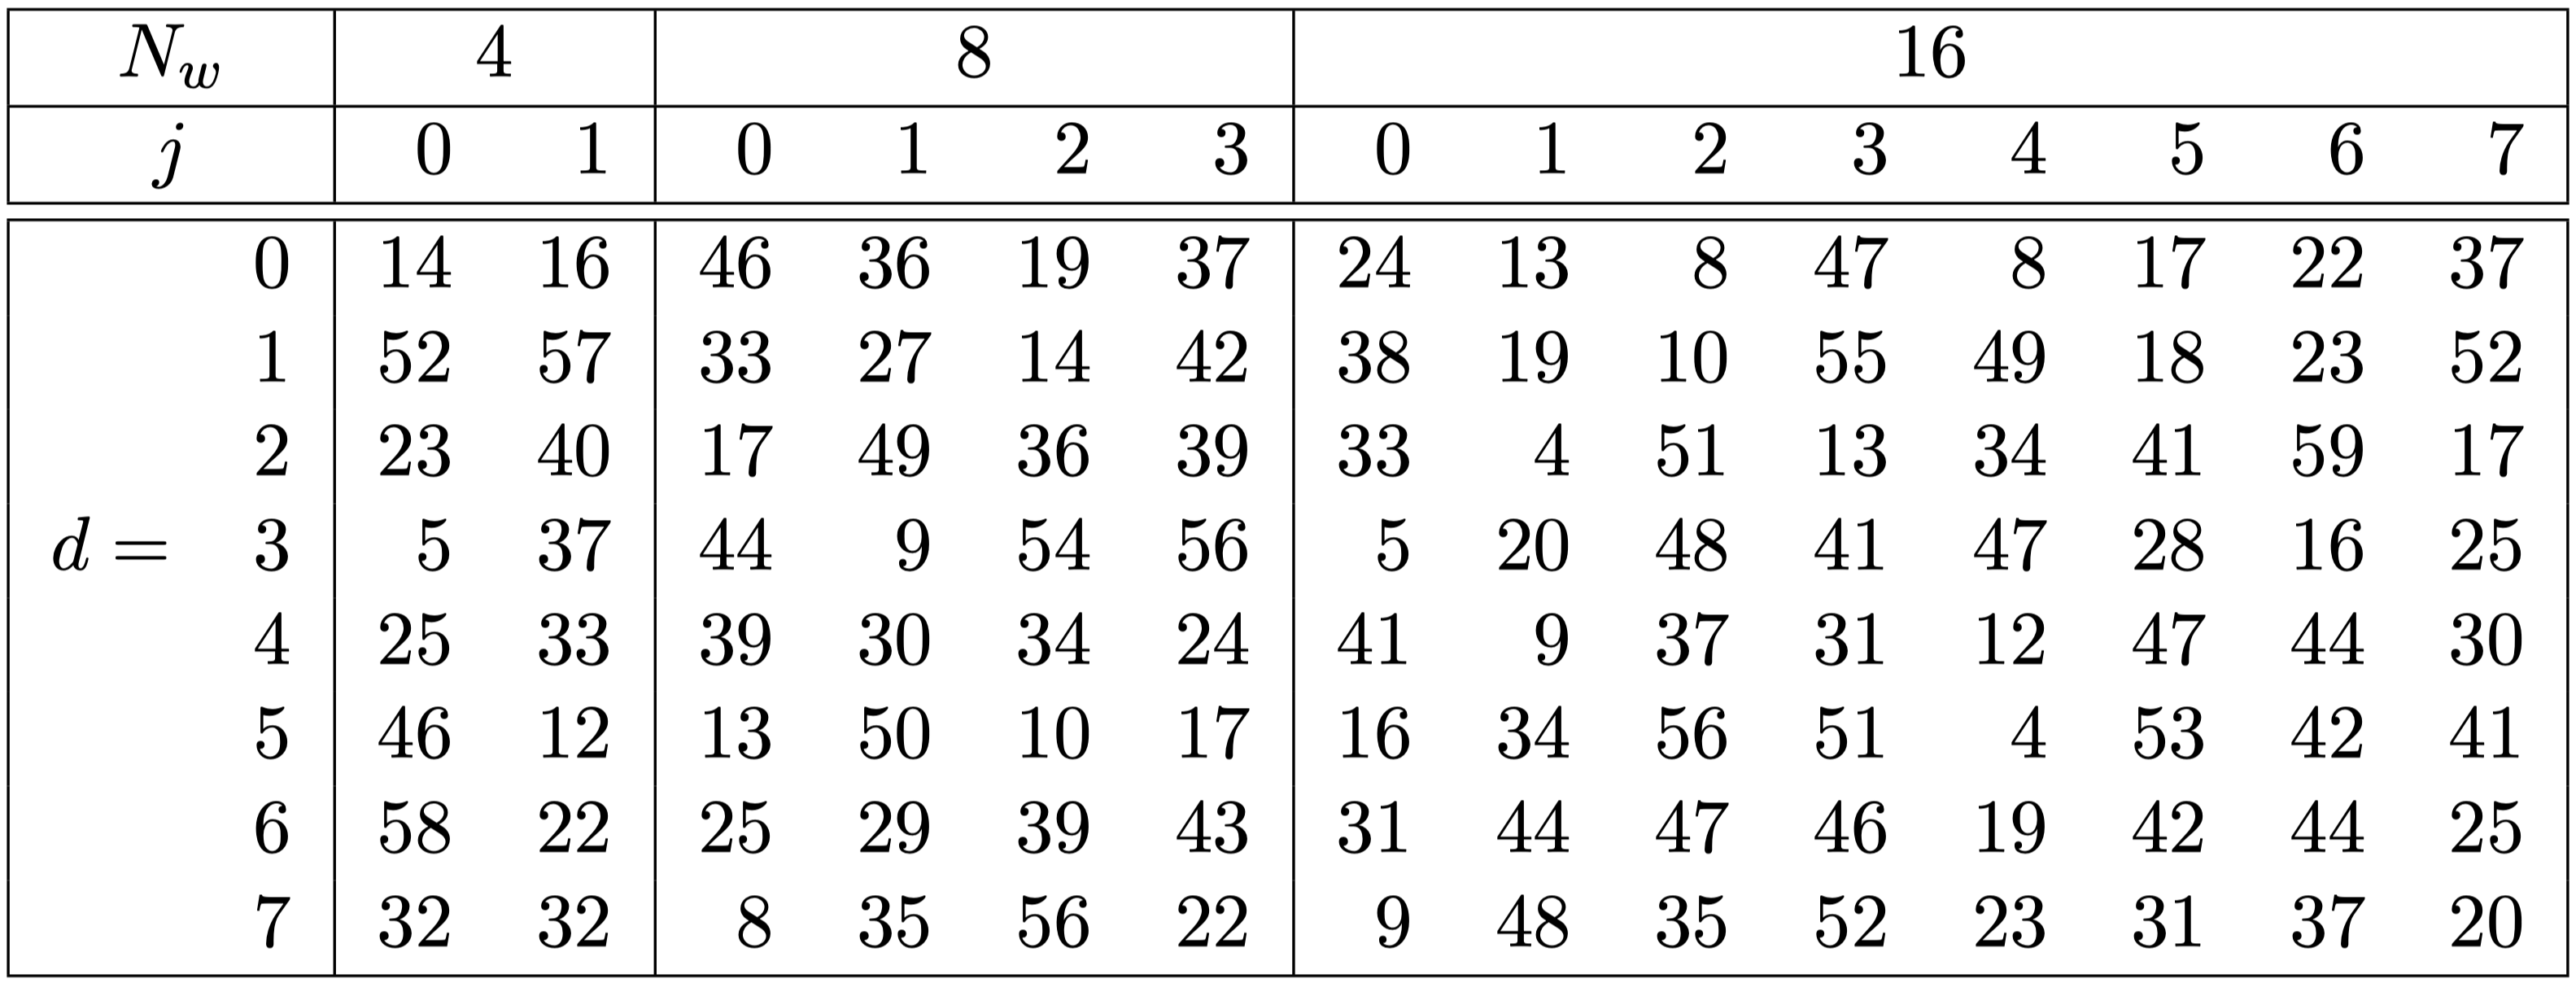
\includegraphics[width=15cm]{Images/Introduction/mix_function_rotate_values.png}	
  	\caption{جدول حاوی تعداد چرخش‌های صورت گرفته در تابع 
  	درهم‌سازی (\lr{Mix})
  }
  \end{figure}

\pagebreak
\subsubsection{
تابع جابه‌جایی (\lr{Permutation})
}
اگر فرض کنیم که خروجی های تابع درهم‌سازی (\lr{Mix}) $j$ در بلاک رمزگذاری $d$ ام، 
$f_{d,\ 2j}$
و
$f_{d,\ 2j+1}$
باشند، خروجی نهایی بلاک رمزگذاری یا در واقع ورودی بلاک رمزگذاری بعدی، برابر خروجی تابع غیر خطی جابه‌جایی (\lr{Permutation}) روی این مقادیر است که از رابطه ی زیر به دست می‌آید:
$$v_{d+1,\ i} = f_{d,\ \pi(i)}$$
که
$v$
معرف بسته‌ی اطلاعاتی ۶۴ بیتی و عدد
 $i$
  شماره‌ی آن بسته در بلاک رمزگذاری مربوط و  $\pi(i)$ یک تابع بوده که مقادیر آن در جدول زیر قابل مشاهده است:

 \begin{figure}[H]
	\centering
	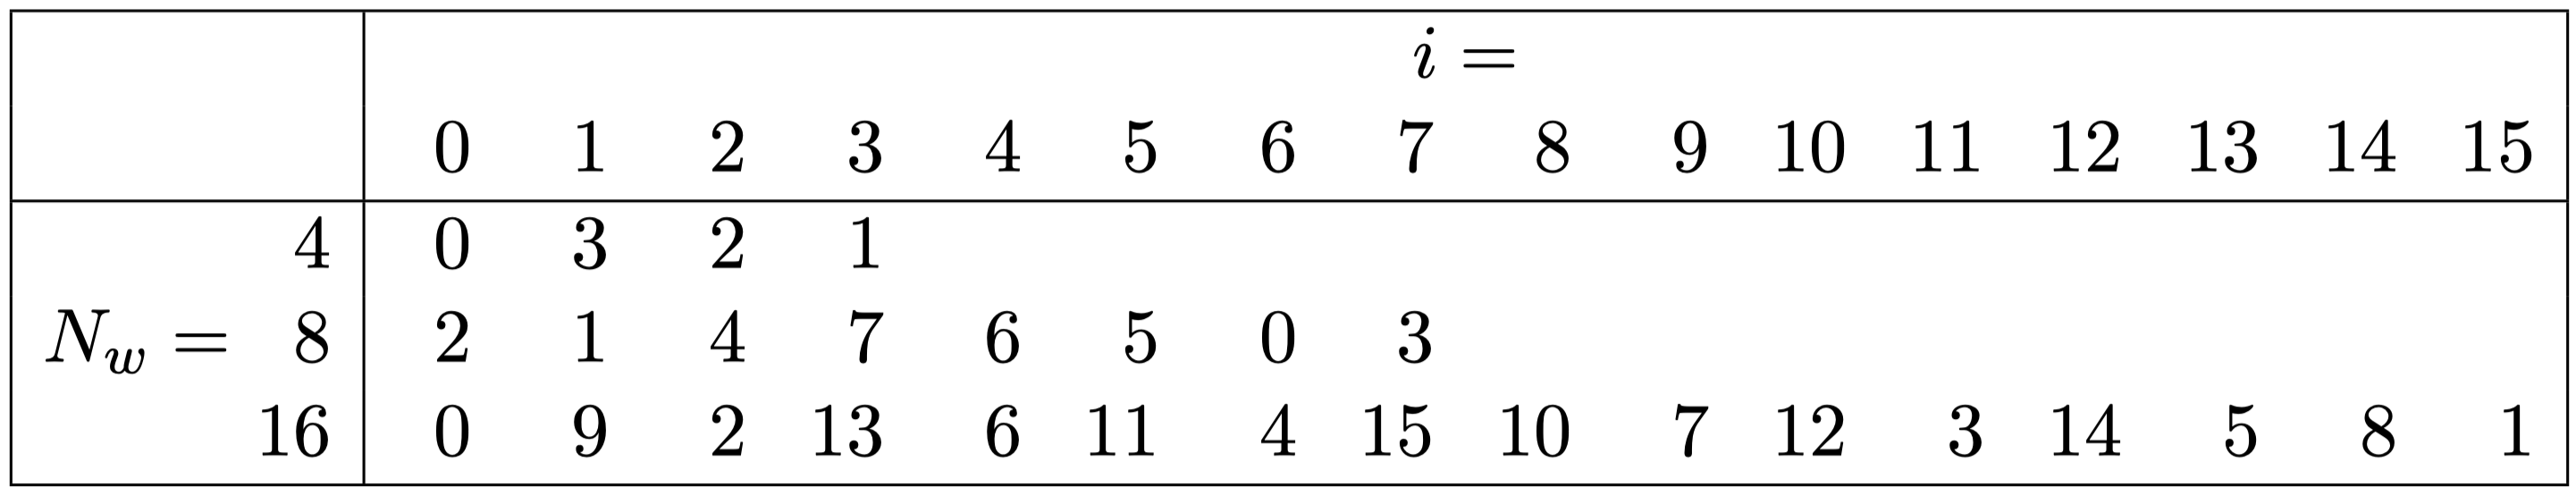
\includegraphics[width=15cm]{Images/Introduction/permutation_values.png}	
	\caption{جدول حاوی مقادیر
	$\pi(i)$
	برای محاسبه‌ی خروجی تابع جابه‌جایی (\lr{Permutation}) 
 }
\end{figure}
  
\subsubsection{
عملیات افزودن مقادیر کلید‌ها 
(\lr{Subkeys})
}

علاوه بر دادگان ورودی ( فرضا 
$p_0$ 
تا
$p_{N_W - 1}$
بسته های ۶۴ بیتی ورودی به کل بخش 
\lr{Threefish}
می‌باشند.
)
مقادیری به عنوان کلیدهای رمزگذاری (
$k_0$ 
تا
$k_{N_W - 1}$
که خود بسته‌های ۶۴ بیتی اند
)
و
دو بسته‌ی ۶۴ بیتی 
$t_0$ 
و
$t_1$
به عنوان تنظیم (
\lr{Tweak}
) 
نیز به ‌بخش 
\lr{Threefish}
در این الگوریتم داده می‌شوند. این مقادیر اضافه پیش از هر ۴ بلاک رمزگذاری با مقادیر خروجی از بلاک رمزگذاری قبل ترکیب می‌شوند. درواقع ورودی بلاک رمزگذاری $d$ ام از رابطه ی زیر به دست می‌آید:
\begin{figure}[H]
	\centering
	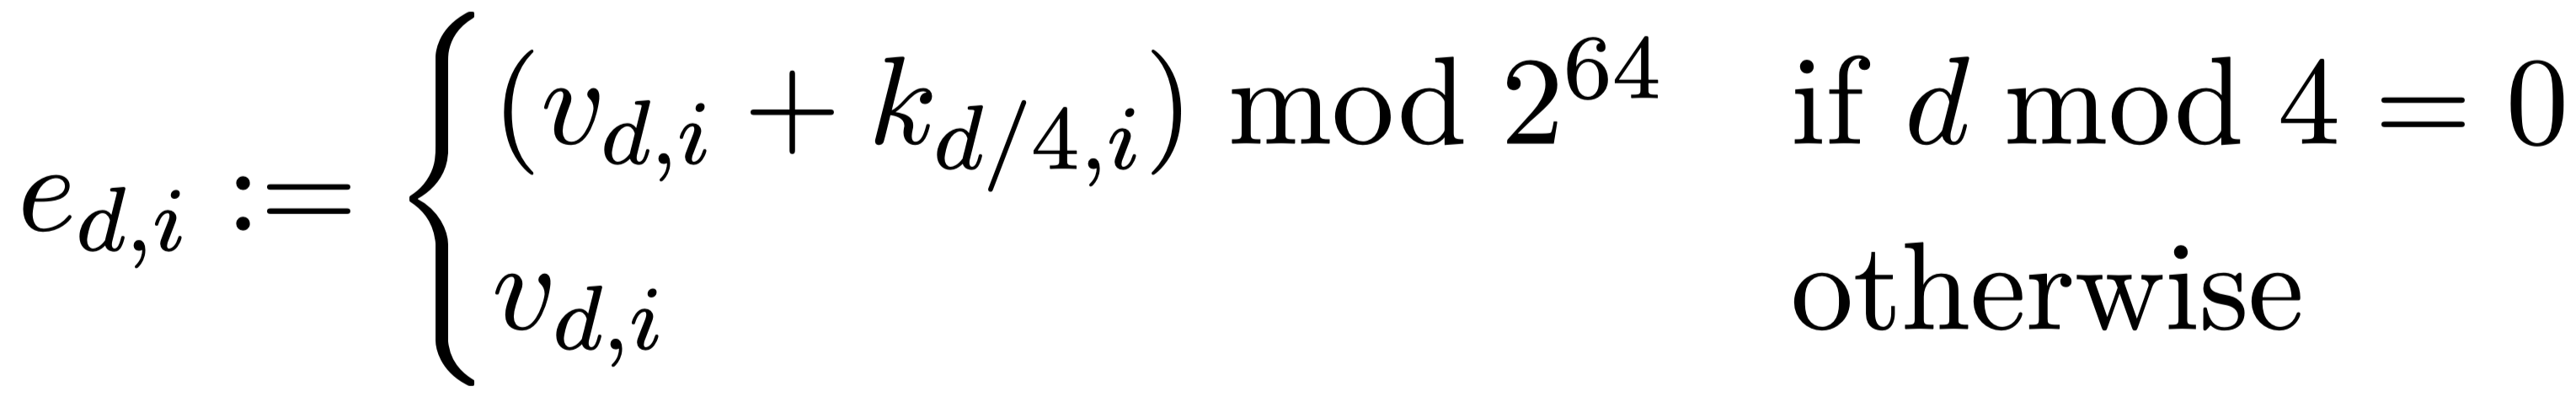
\includegraphics[width=7cm]{Images/Introduction/subkey_equation_1.png}	
	
\end{figure}
که $i$ در شماره‌ی بسته‌ی ۶۴ بیتی اطلاعات است و $v_{0,i}$ ها همان بسته های ۶۴ بیتی ورودی به کل بخش 
\lr{Threefish}
یعنی 
$p_0$ 
تا
$p_{N_W - 1}$
می‌باشند  و مقدار $k$ ها نیز با‌توجه به روابط زیر قابل مقایسه است:
	\begin{latin}
		\begin{center}
			\begin{tabular}{l l}
				$k_{s, i} = k_{(s+i) \mod\ N_W+1} $ \hspace{15mm} & $  i = 0,\ 1,\ 2,\ ... ,\ N_W-4 $ \\
				$k_{s, 5} = k_{(s+5) \mod\ N_W+1} + t_{s \mod 3}$ & \\
				$k_{s, 6} = k_{(s+6) \mod\ N_W+1} + t_{(s+1) \mod 3}$ & \\
				$k_{s, 7} = k_{(s+7) \mod\ N_W+1} + s $ & \\
				
			\end{tabular}
		\end{center}
	\end{latin}

که در این روابط مقادیر $k_{N_W}$ و
$t_2$
از قرار زیر اند:
$$
k_{N_W} = C_{240} \oplus k_0 \oplus k_1 \oplus ... \oplus k_{N_W - 1}
$$

$$
t_2 = t_1 \oplus t_0
$$
که $ C_{240} $ عددی ثابت و برابر \lr{0x1BD11BDAA9FC1A22} است و به آن جهت در فرمول وجود دارد که از ۰ نبودن تمامی بیت‌ها اطمینان حاصل شود.

\subsection{
	\lr{Unique Block Iteration (UBI)}
}

\subsection{
	\lr{Optional Argument System}
}

	\chapter{
	پیاده‌سازی سخت‌افزاری با
	\lr{Verilog}
}

\section{
	مقدمه
}

دنیای نرم‌افزار و سخت‌افزار رایانه در نگاه کلی می‌توانند بسیار شبیه به هم باشند، برنامه های نرم‌افزاری، مقادیری را به عنوان ورودی دریافت کرده، سپس طی روند مشخصی محاسباتی روی آنها انجام داده و در نهایت مقادیری را به عنوان خروجی به کاربر خود تحویل می دهند، قطعات سخت‌افزاری نیز دارای 
\lr{port}
هایی برای ارتباط با دنیای خارجی و دریافت ورودی‌ و تحویل خروجی‌های خود می‌باشند و از واحدهای مختلف پردازشی و عملیاتی مختلفی برای محاسبه ی خروجی‌های مناسب تشکیل شده اند. درعمل می‌توان سخت‌افزاری خاص برای اجرای بسیاری از روند های نرم‌افزاری طراحی و پیاده سازی کرد، ساخت سخت‌افزارِ خاصِِ مربوط به یک الگوریتم می تواند کاربرد‌های بسیاری داشته باشد، برای مثال قطعه‌ای که بتواند داده های ورودی را رمزنگاری کند می‌تواند به صورت گسترده برای ذخیره ی اطلاعات به صورت سریع استفاده شود، سخت‌افزار های اختصاصیِ الگوریتم ها سریع و بهینه اند و میتوانند به اجرای هرچه سریع تر روندهای پیچیده‌ای که به الگوریتم مورد نظر وابستگی فراوان دارند کمک کلانی کنند.

همانند بسیاری از الگوریتم‌های رایانه‌ای، الگوریتم تابعِ 
\lr{
	Skein Hashing
}
که در بخش قبل کلیتی از آنرا معرفی کردیم را می توان به صورت سخت افزاری پیاده‌سازی کرد، بدین صورت که قطعه‌ای طراحی و پیاده‌سازی کنیم که ورودی ای به اندازه ی دلخواه مارا دریافت و حاصل درهم‌سازی را به صورت خروجی ای به اندازه ی مورد نظر ما خروجی دهد. بر اساس نیاز و کاربرد ما از این قطعه، اندازه‌ی ورودی و خروجی را می توان ثابت و به مقدار دلخواه درنظر گرفت، سپس قطعه‌ای ثابت با پیاده سازیِ بهینه‌ای برای اندازه های مورد نظر طراحی کرد، یا این که قطعه‌ای  برای ورودی و خروجی های با اندازه های متغیر طراحی و پیاده سازی کرد. همان طور که در بخش قبل توضیح داده شد، تابع درهم‌سازی 
\lr{
	Skein Hashing
}
میتواند ورودی‌ای با اندازه ی دلخواه را دریافت کند و خروجی ای با اندازه‌ی دلخواه تحویل دهد، در این مقاله تمرکز ما روی پیاده سازی سخت‌افزاری حالتی از این تابع می باشد که اندازه ی بلاک های درونی تابع ( حالت درونی تابع ) 
\textbf{۵۱۲ بیت}
و حاصل درهم‌سازی نیز به صورت خروجی ای به اندازه ی 
\textbf{۵۱۲ بیت}
می باشد، این تابع در اصطلاح 
\lr{
	\textit{Skein 512-512}
}
نامیده می‌شود.

مراحل طراحی و پیاده‌سازی سخت‌افزاری یک قطعه معمولا به آن صورت است که برای اطمینان از کارکرد صحیح پیاده‌سازی، موازی با طراحی سخت‌افزاری قطعه، پیاده سازی دیگری از الگوریتم به نام مدل طلایی انجام می‌شود و پس از پایان طراحی‌ها، کارکرد قطعه با مدل طلایی مقایسه می شود تا قطعه‌ی نهایی مشکلی نداشته باشد. در بخش 
\hyperref[chapter:GoldenModel]{\textbf{مدل طلایی}}
به تفصیل درباره‌ی مدل طلایی استفاده شده در این پروژه توضیح داده شده است. در این بخش به پیاده‌سخت‌افزاری این الگوریتم به کمک زبانِ توصیف سخت‌افزارِ 
\lr{Verilog}
می پردازیم.

\pagebreak
\section{
	پیاده‌سازی
}
همان طور که توضیح داده شد، الگوریتم 
\lr{Skein}
از سه بخش اصلی تشکیل می‌شود:
\begin{itemize}
	\item 
	\lr{\textit{\textbf{Threefish}}} 
	یا بلاک های رمزنگاری قابل تنظیم،
	\item
	\lr{
		\textit{
			\textbf{Unique Block Iteration (UBI)}
		}
	}
که یک حالت زنجیره ای است که از
\lr{Threefish}
به صورتی استفاده می کند که ورودیِ ‌به اندازه‌ی دلخواه به خروجی‌ای به اندازه‌ای مشخص تبدیل شود.
\item
\textbf{\lr{\textit{\textbf{Optional Argument System}}} } 
که به الگوریتم توانایی پشتیبانی از بسیاری ویژگی های دلخواه را، بدون افزودن باری اضافه به پیاده سازی الگوریتم می‌دهد.

\end{itemize}

طراحی ای که ما در این پروژه به بررسی‌اش می‌پردازیم، یک طراحی بسیار ساده شده از الگوریتمِ
\lr{Skein 512-512}
می باشد. در این طراحی اندازه ی ورودیِ و خروجی اش ثابت و ۵۱۲ بیت می باشند، و اندازه ی حالت درونی تابع درهم‌سازی نیز دقیقا برابر اندازه‌ی ورودی و خروجی‌هاست، بنابراین در این طراحی اثری از پیاده‌سازی یک 
\lr{UBI}
 پیچیده نیست. علاوه‌ بر این، این پیاده‌سازی، پیاده‌سازی خام خود الگوریتمِ
 \lr{Skein 512-512}
 بوده و هیچ ویژگی اضافی ای را پشتیبانی نمی‌کند، بنابراین اثری از پیاده‌سازی 
\lr{Optional Argument System}
نیز در آن نیست. بنابراین طراحی، صرفا شامل بلاک های رمزنگاری قابل تنظیم بوده، داده‌ی ورودی به صورت مستقیم با این بلاک ها تزریغ شده و خروجی الگوریتم نیز به صورت تقریبا مستقیم از آخرین بلاک دریافت می‌شود.

\subsection{
	بررسی درستی طراحی ارائه شده
}
طراحی‌ای که دراختیار ما قرار گرفته بود 
(
\href{https://github.com/VahidZee/SkeinHashingHDL/blob/master/SourceCode/Verilog/skein.v}{این فایل} 
)
، شامل مشکلات منطقی فراوان بود، مشکلات موجود در هر خط از کد 
\lr{verilog}
به صورت یک 
\lr{comment}
در قالب 
$$todo: <Valid Code>$$
مشخص شده اند، علاوه بر این طراحی تصحیح شده 
(
\href{https://github.com/VahidZee/SkeinHashingHDL/blob/master/SourceCode/Verilog/corrected.v}{این فایل} 
)
نیز در کنار مقاله پیوست شده است، تمامی مستند سازی های این مقاله، براساس پیاده سازی تصحیح شده ی کدهای اولیه می‌باشد.
\subsection{
	ساختار طراحی
}
ساختار کلی طراحی شده برای این الگوریتم به سه بخش که در تصویر زیر قابل مشاهده اند قابل تفکیک است، ماژول اصلی طراحی که 
\lr{skein512}
نام گذاری شده است، این سه وظیفه را بر‌عهده دارد.
\vspace{-0.2cm}
\begin{figure}[H]
	\centering
	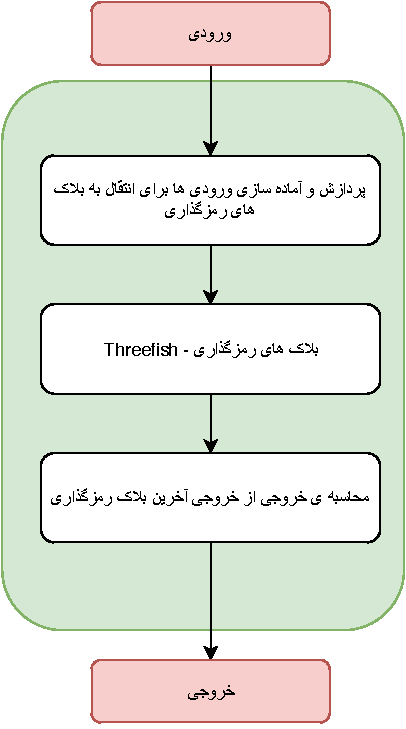
\includegraphics[width=3.5cm]{Images/VerilogDocumentation/skein_functionality.pdf}	
	\caption{ساختار کلی پیاده‌سازی سخت‌افزاری}
\end{figure}
دو بخش پردازش ورودی و خروجی‌ها به صورت کامل در ماژول 
\lr{skein512}
صورت می گیرند و به تفصیل درباره ی آنها توضیح داده خواهد شد، بخش بلاک های رمزگذاری از ماژول های 
\lr{skein\_round} 
و 
\lr{skein\_round\_1} 
تا 
\lr{skein\_round\_4} 
تشکیل شده و قرارگیری زنجیره‌ای آنها و محاسبه ی اولیه‌ی مقادیر کلید‌های رمزنگاری در ماژول 
\lr{skein512}
صورت گرفته است.

\subsection{
	پیاده سازی بلاک‌های رمزگذاری
}
همان‌طور که در معرفی الگوریتمِ
\lr{Skein Hashing}
در بخش اول توضیح داده شد، این الگوریتم برای تولید مقدار درهم‌سازی از بلاک های رمزگذاری که به صورت زنجیره ای یکی پس از دیگری قرار گرفته اند، استفاده می کند و این بلاک‌ها بخش عمده‌ای از طراحی سخت‌افزاری را دربر می‌گیرند. 

شمای کلی حرکت داده داخل بلاک های رمزنگاری در این الگوریتم به شکل زیر می باشد:
\begin{figure}[H]
	\centering
	\includegraphics[width=7cm]{Images/VerilogDocumentation/cipherblock_dataflow.png}	
	\caption{شمایی از حرکت داده در بلاک های رمزنگاری}
\end{figure}
داده‌ی ورودی که به ۸ بخشِ ۶۴ بیتی تقسیم می‌شود، به بلاک‌های رمزنگاری تزریق شده و پس از ۴ مرحله ی متوالی از درهم‌سازی 
(
\lr{Mix}
)
و
 جابه‌جایی 
 (
 \lr{Permutation}
 )
 - که به هر‌ یک از آنها یک
 \lr{\textit{round}}
 می‌گوییم -  
 با مقادیری به نام 
\lr{\textit{Subkey}}
که از کلید‌های رمزنگاری - که آنها نیز از ۸ بلاک ۶۴ بیتی تشکیل شده اند - به دست می‌آیند، جمع می‌شوند.

محاسبات دقیق
\lr{Subkey}
ها و توابعِ غیرخطی 
درهم‌سازی 
(
\lr{Mix}
)
و
جابه‌جاییِ 
(
\lr{Permutation}
)
 هر
\lr{round}
به تفصیل در بخش اول مقاله، توضیح داده شده است. آن چیزی که در‌این میان حائز اهمیت است، استفاده‌ای هوشمندانه از نظم تکراری این توابع محاسباتی در پیاده‌سازی سخت‌افزاری مورد بررسی ما در این مقاله است.
\pagebreak

\subsubsection{
	پیاده سازی توابع جابه‌جایی 
	(
	\lr{Permutation}
	)
	هر
	\lr{round}
}
 تابع غیرخطیِ جابه‌جایی
(
\lr{Permutation}
)
یک عملیات ثابت را روی مقادیر خروجی از توابع درهم‌سازی
(
\lr{Mix}
)
انجام می‌دهد، این تابع در ماژول‌های 
\lr{skein\_round\_1} 
تا 
\lr{skein\_round\_4} 
به صورت توصیف رفتاری با کمک یک 
\lr{always block}
حساس به لبه‌ی بالا‌رونده‌ی ساعت پیاده سازی شده است.
مقادیر خروجی توابع درهم‌سازی (
\lr{Mix}
)
مربوط به هر ماژول - که جلوتر پیاده‌سازی آنها را بررسی خواهیم کرد -، به هنگام لبه‌ی بالارونده ی ساعت، جابه‌جا شده و به خروجی ماژول انتقال داده می‌شوند. 


توصیف ارائه شده از جابه‌جایی 
(
\lr{Permutation}
)
در این 
\lr{always block}
ها در واقع معرف مجموعه ای از ۵۱۲ 
\lr{D-FlipFlop}
 حساس به لبه‌ی بالا‌رونده ی ساعت می باشد.
 
 \subsubsection{
 پیاده سازی توابع درهم‌سازی 
 (
 \lr{Mix}
 )
 هر
 \lr{round}
}
برخلاف توابع جابه‌جایی (
\lr{Permutation}
) که یک عملیات ثابت را در هر 
\lr{round}
اجرا می‌کنند، این توابع غیر‌خطی، بر اساس این که در کدام
\lr{round}
قرار دارند،‌ محاسبات خاص خود را خواهند داشت، همان طور که در بخش قبل توضیح داده شد، هر درهم‌سازی (
\lr{Mix}
) شامل، یک جمع، یک گردش به چپ و یک
\lr{xor}
می باشد. جمع و \lr{xor} ها در همه‌ی \lr{round} ها یکسان‌ اند و به صورت یکتا پیاده می‌شوند.

 چیزی که در هر
 \lr{round}
  متفاوت خواهد بود، تعداد گردش ها به چپ می‌باشد،
با توجه به مقادیر ارائه شده و فورمول‌های توضیح داده شده در بخش قبل، این مقادیر هر ۸ 
\lr{round}
 تکرار می شوند، مسئله ی دیگر آن است که قرار است هر ۴ 
 \lr{round}
 ،
\lr{subkey}
   های مربوطه به مقادیر موجود در بلاک‌های رمزگذاری افزوده شوند، برای همین در پیاده‌سازی مورد بررسی ما هر ۴ 
\lr{round}
   در یک ماژول به نام
    \lr{skein\_round}
    در نظر گرفته شده است و پیاده سازی خود 
     \lr{round} 
     ها در ماژول های  
     \lr{skein\_round\_1} 
     تا 
     \lr{skein\_round\_4} 
     تعریف شده اند.
     این بدین معنا است که برای دوره ی تناوب ۸ تایی توابع درهم‌سازی (
     \lr{Mix}
     ) هر 
     \lr{round}
     ، صرفا دانستن این که در ۴  \lr{round} شماره ی فرد یا زوج قرار داریم برای ماژول های 
     \lr{skein\_round\_1} 
     تا 
     \lr{skein\_round\_4} 
     کافی می باشد. برای همین این ماژول‌ها یک ورودی تک بیتی به نام
     \lr{even}
     دریافت می کنند و بر اساس آن تعداد گردش به چپ‌های مناسب را بر می گزینند.
     
     پیاده‌‌سازی خود توابع درهم‌سازیِ (
     \lr{Mix}
     ) هر 
     \lr{round}
   ، در دو بخش در ماژول های 
    \lr{skein\_round\_1} 
    تا 
    \lr{skein\_round\_4} 
تعریف شده است.
در بخش اول عملیات‌های جمع و گردش به چپ‌ها به توصیفی ساختاری و به کمک یک سری 
\lr{continuous assignment} 
در این ماژول‌ها مشخص شده‌ اند، لازم به ذکر است که در 
\lr{verilog}
عملگر گردش به چپ وجود ندارد، برای همین برای پیاده سازی گردش به چپِ یک \lr{vector}، از ترکیب \lr{part selection} و \lr{concatenation} استفاده شده است.
 در بخش دوم عملیات‌های
\lr{xor}
هم‌زمان با عملیات‌های جابه‌جایی (
\lr{Permutation}
)
در 
\lr{always block}
مربوط به آنها در این ماژول‌ها معرفی شده است.

توصیف ارائه شده از توابع درهم‌سازی (
\lr{Mix}
) 
در عمل معرف مجموعه ای از مدار‌های ترکیبی (
\lr{combinational}
) می باشد و منجر به تولید گیت‌های منطقی مستقل از سیگنال ساعت خواهد شد.

\subsubsection{
	پیاده سازی 
	\lr{round}
	ها
}
همان طور که بار ها گفته شد \lr{round} شامل درهم‌سازی 
(
\lr{Mix}
)
و
جابه‌جاییِ 
(
\lr{Permutation}
)
روی ورودی‌هایش می‌باشد که به تفصیل به پیاده سازی این دو تابع غیرخطی در طراحی مورد بررسی‌مان پرداختیم، تنها مسئله ی مجهول شیوه‌ی اتصال این دو بخش در ماژول های 
 \lr{skein\_round\_1} 
تا 
\lr{skein\_round\_4} 
و تشکیل واحد های محاسباتی \lr{round} های الگوریتم می‌باشد که بلاک دیاگرام های تهیه شده در تصاویر دو صفحه‌ی بعدی به تفصیل این مسئله و هم‌چنین شمای کلی حرکت داده داخل این ماژول‌ها را توضیح می دهند:
\begin{figure}[H]
	\centering
	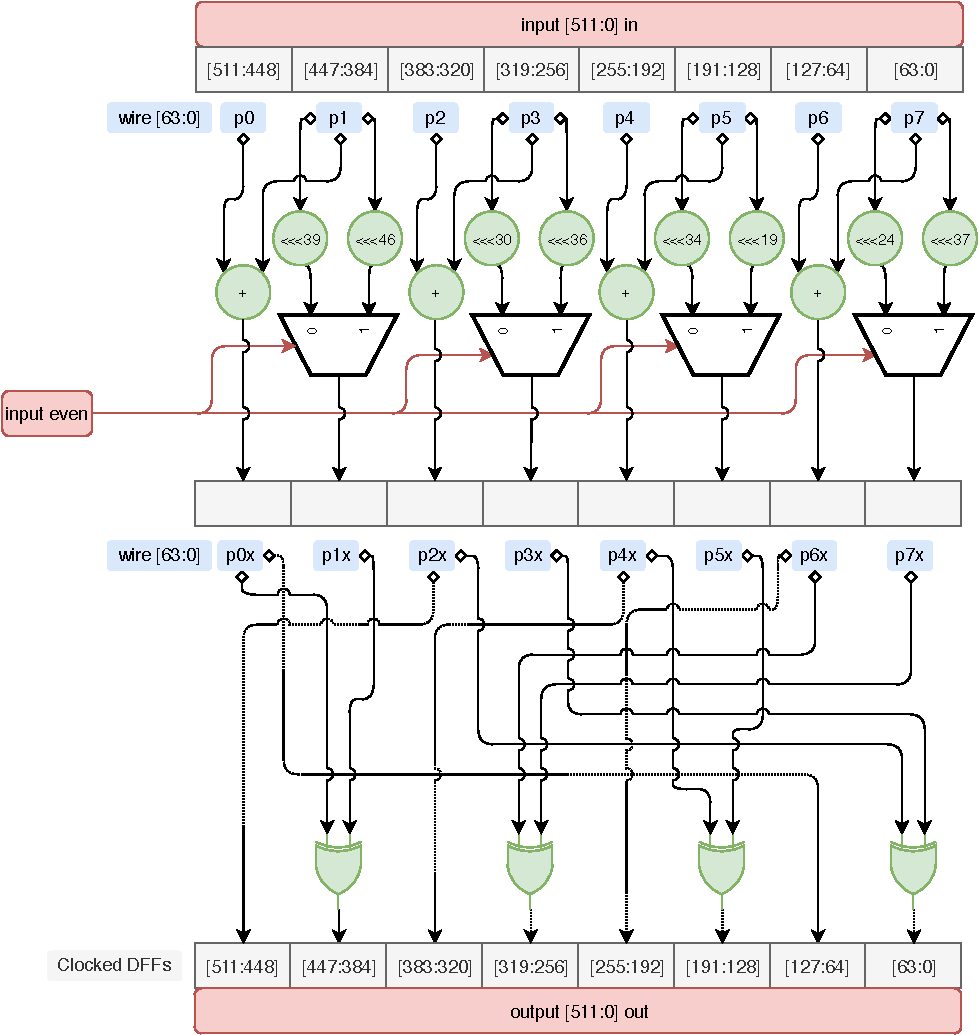
\includegraphics[width=10.5cm]{Images/VerilogDocumentation/diagrams_round1.pdf}	
	\caption{
	بلاک دیاگرام شماتیک و نحوه‌ی جریان داده در ماژول 
	\lr{skein\_round\_1}
}
\end{figure}
\begin{figure}[H]
	\centering
	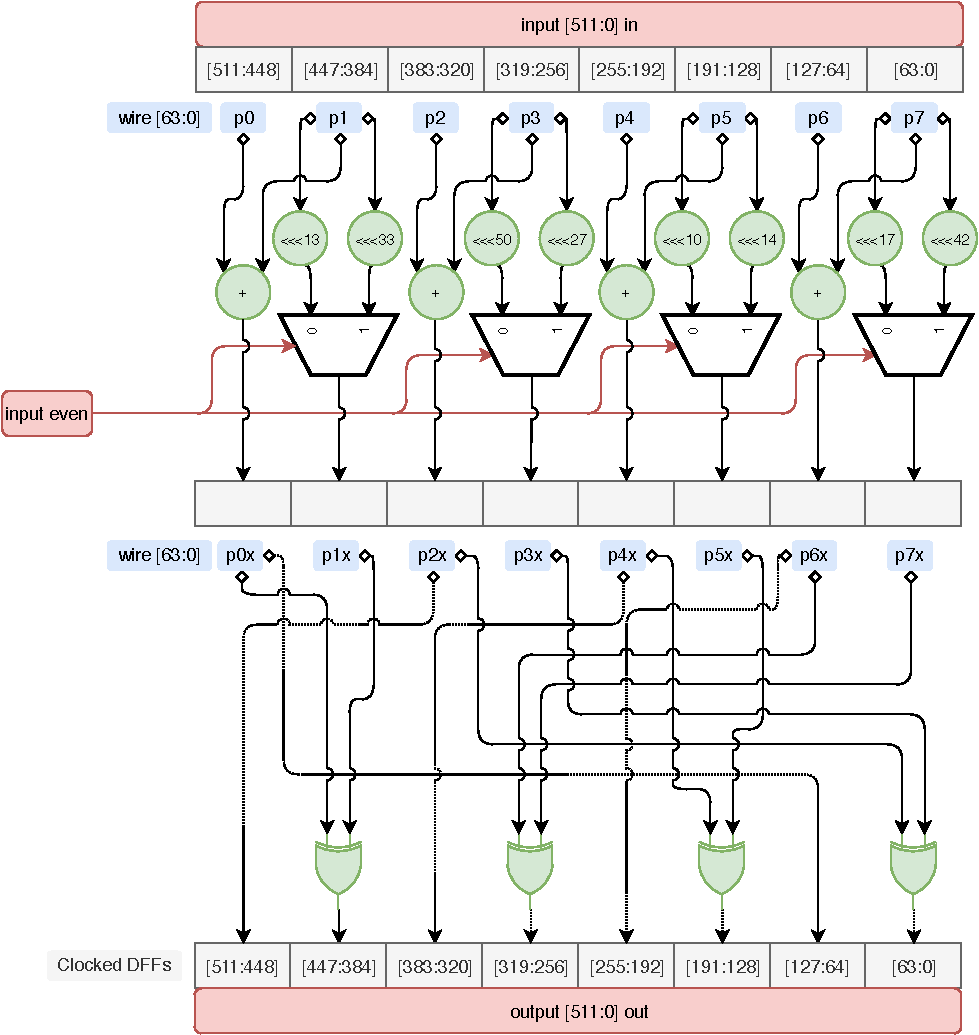
\includegraphics[width=10.5cm]{Images/VerilogDocumentation/diagrams_round2.pdf}	
	\caption{
		بلاک دیاگرام شماتیک و نحوه‌ی جریان داده در ماژول 
		\lr{skein\_round\_2}
	}
\end{figure}
\begin{figure}[H]
	\centering
	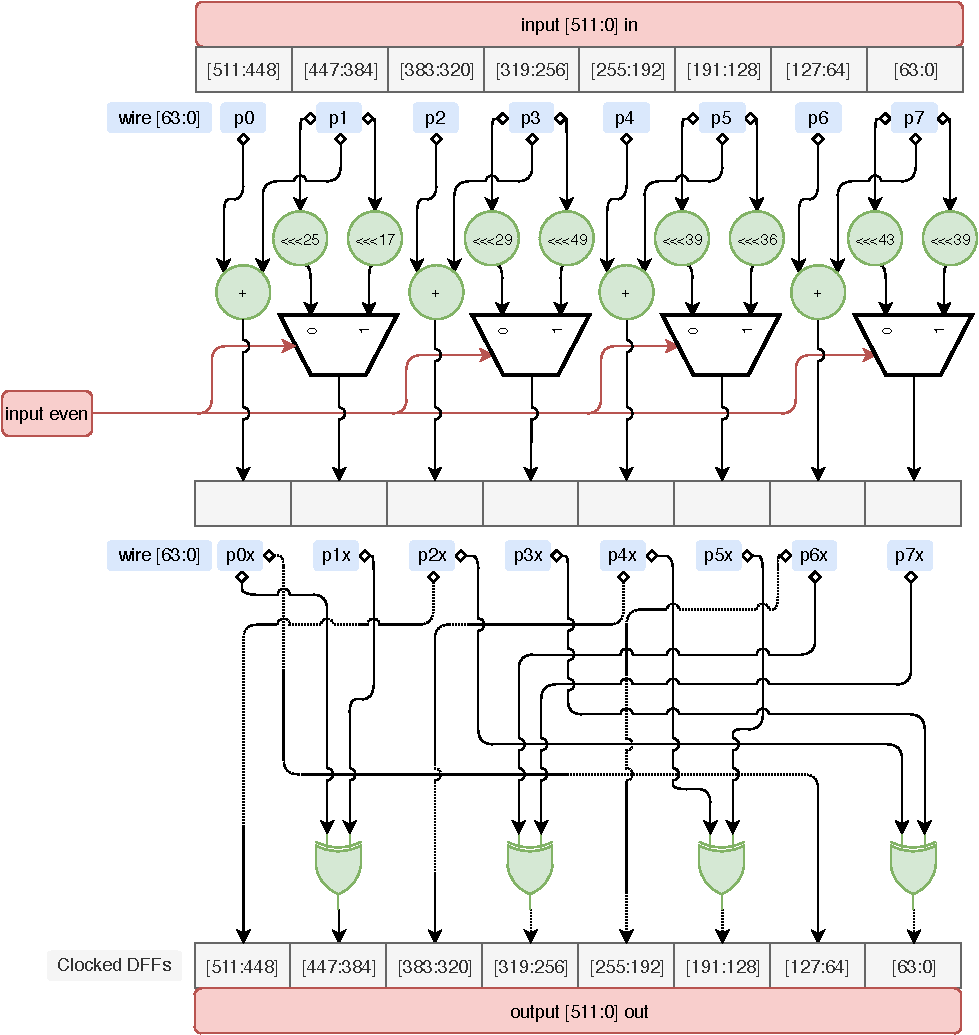
\includegraphics[width=10.5cm]{Images/VerilogDocumentation/diagrams_round3.pdf}	
	\caption{
		بلاک دیاگرام شماتیک و نحوه‌ی جریان داده در ماژول 
		\lr{skein\_round\_3}
	}
\end{figure}
\begin{figure}[H]
	\centering
	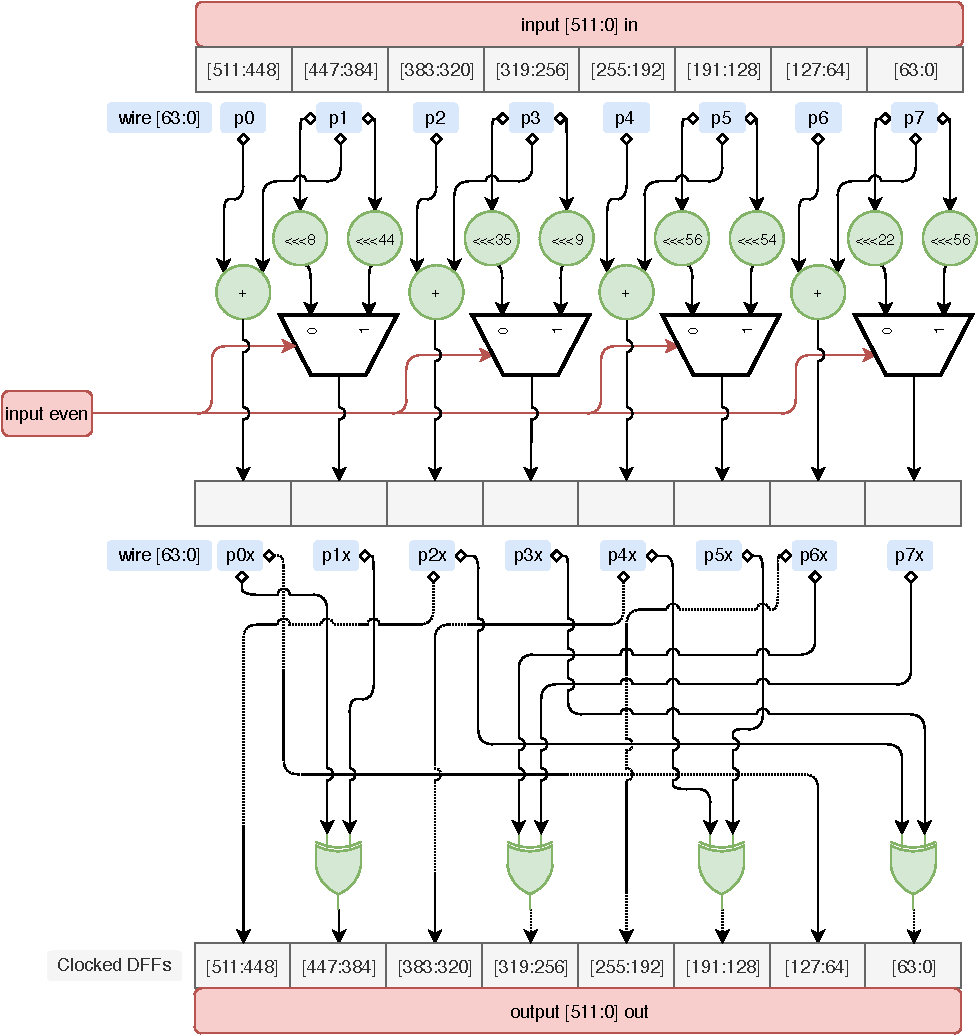
\includegraphics[width=10.5cm]{Images/VerilogDocumentation/diagrams_round4.pdf}	
	\caption{
		بلاک دیاگرام شماتیک و نحوه‌ی جریان داده در ماژول 
		\lr{skein\_round\_4}
	}
\end{figure}

\subsubsection{
	محاسبه و افزودن 
	\lr{Subkey}
	ها
}
همان‌طور که اشاره شد، قبل از هر ۴
\lr{round}
مقادیری به نام 
\lr{Subkey}
به مقادیر محاسبه شده در بلاک‌های رمزگذاری افزوده می‌شود، طبق توضیحات بخش اول، مقادیر 
%todo reference
\lr{Subkey}
‌ها باتوجه به شماره‌ی
\lr{round}
تنظیم می‌شوند، اگر به فورمول محاسبه‌ی 
\lr{Subkey}
ها توجه کنید
%todo formula refrence
متوجه دو تناوب خواهید شد، یکی برای خود مقادیر 
\lr{Subkey}
ها که پس از هر‌بار محاسبه‌، انگار که یک خانه جا‌به‌جا شوند، دیگر آنکه پس از هر‌ ۳ 
\lr{round}
جای مقادیر تنظیم
\lr{tweak} 
(
$t_0$ , $t_1$ , $t_2$
)
یک دور کامل می‌چرخند.

ماژول 
\lr{skein\_round}
 شامل ۴ 
 \lr{round}
 متوالی از بلاک‌های رمزگذاری و واحد افزودن مقادیر 
 \lr{Subkey}
 ها به مقادیر محاسبه شده در بلاک‌های رمزگذاری قبلی و هم‌چنین پیاده‌سازیِ یکی از این دو دوره‌ی تناوب می‌باشد. 
 به صورت خلاصه تصویر زیر معرف شمای کلی و نحوه‌ی جریان داده ها در هر نمونه از ماژول‌های
 \lr{skein\_round}
 می‌باشد:
 \begin{figure}[H]
 	\centering
 	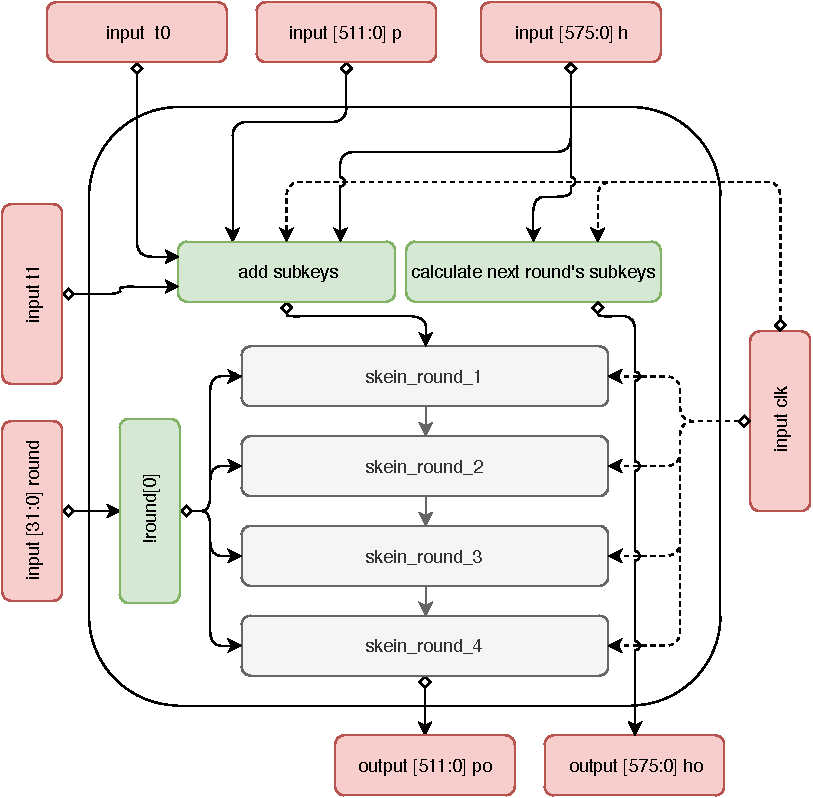
\includegraphics[width=10cm]{Images/VerilogDocumentation/skeinround_dataflow.pdf}	
 	\caption{شمایی از نحوه‌ی حرکت داده و ساختار هر نمونه از ماژول
 	\lr{skein\_round}
 }
 \end{figure}
ورودی 
\lr{input [575:0] h}
به ترتیب از سمت با‌ارزش‌ترین بیت، شامل
\lr{Subkey}
های مربوط به این 
 \lr{round}
 یعنی:
 $$Subkey_{round,\ 0}, Subkey_{round,\ 1}, Subkey_{round,\ 2}, ..., Subkey_{round,\ 8}$$
و ورودی های 
\lr{input t0}
و
\lr{input t1}
به ترتیب حاوی مقادیر تنظیم (
\lr{tweak}
)
مربوط به این 
 \lr{round}
، یعنی:
$$t0 = t_{ round \ mod \ 3 } $$
$$t1 = t_{ (round + 1 ) \ mod \ 3}$$
 می باشد. بنابراین این ورودی ها بدون هیچ پیش‌پردازشی آماده‌ی تزریق به بخش افزایش به مقادیر رمزگذاری شده در 
 \lr{round}
 های قبلی می‌باشند.  بخش افزاینده‌ی مقادیر 
\lr{Subkey}
ها به مقدار رمزگذاری شده از بلاک‌‌(ها)ی قبلی ، در این ماژول،  با توجه به فورمول محاسباتی توضیح داده شده در بخش قبل، محاسبات مربوط به این 
 \lr{round}
 را از روی ورودی های خود انجام می‌دهد. 
پیاده‌سازی این بخش در کد با توصیفی رفتاری به کمک یک 
\lr{always block}
حساس به لبه‌ی بالارونده‌ی ساعت مشخص شده است. این توضیحات بخش اول توصیفات موجود در این 
\lr{always block}
بوده و در عمل معرف ترکیبی از یک مداری ترکیبی (‌برای محاسبات جمع 
\lr{Subkey} 
ها‌و مقادیر رمزگذاری شده‌ي 
\lr{p}
) و مداری ترتیبی (برای انتقال حاصل عملیات‌های جمع به ورودی 
\lr{skein\_round\_1}
) می‌باشد.

بخش دیگری که در این ماژول پیاده‌سازی شده است، محاسبه‌ی 
\lr{Subkey}
های مربوط به
 \lr{round}
 بعدی براساس 
 \lr{Subkey}
 های این 
  \lr{round}
  می‌باشد.
  اگر به فورمول های محاسبه‌ی
  \lr{Subkey}
  ها توجه کنید، واضح است که پس از هر 
   \lr{round}
   انگار  \lr{Subkey}
   ها یک گردش به چپ دارند. دقیقا همین ایده در این ماژول به کمک توصیفی رفتاری در بخش دوم کد های 
   \lr{always block}
   حساس به لبه‌ی بالارونده‌ی ساعت، پیاده شده‌است. این توصیف در واقع معرف یک مدار ترکیبی برای محاسبه ی حاصل 
   \lr{xor}
   $Subkey_{round,\ 0}$
   تا
$Subkey_{round,\ 7}$
و یک مدار ترتیبی برای انتقال مقادیر یک بلاک چرخش به چپ و حاصل 
\lr{xor}
\lr{Subkey}
ها به خروجی می باشد.

پیاده‌سازی و مقدار‌دهی تناوبی مقادیر تنظیم (
\lr{tweak}
)
به هنگام نمونه‌گیری ماژول‌های 
\lr{skein\_round}
در ماژول اصلی یعنی
\lr{skein512}
انجام شده است.

\subsubsection{
	اتصال 
	\lr{round}
	ها به یکدیگر و پیاده‌سازی بلاک های رمزگذاری به صورت زنجیره‌ای
}
در پیاده‌سازی الگوریتم
\lr{Skein 512-512}
برای محاسبه‌ی مقدار درهم‌سازی نهایی باید ۷۲ 
\lr{round}
بلاک‌های رمزگذاری پشت‌سر‌هم به صورت یک زنجیره تکرار شوند، پیاده‌سازی این مسئله در ماژول 
\lr{skein512}
که بالاترین ماژول طراحی مورد بررسی ما است، صورت می‌گیرد.

این‌کار به صورت ترکیبی از توصیف های ساختاری و رفتاری در این ماژول انجام شده است،
کنارهم قرارگرفتن بلاک‌های رمزگذاری به توصیفی ساختاری با نمونه گیری از ۱۸ ماژول 
\lr{skein\_round}
انجام شده است. همان‌طور که در بخش قبل توضیح داده شد، محاسبات مربوط به 
\lr{Subkey}
ها، دارای دو تناوب هستند، یکی از این تناوب ها در محاسبات داخل خود ماژول های 
\lr{skein\_round}
صورت می‌گیرد که به تفصیل درباره‌ی آن توضیح داده شد. تناوب دومِ محاسباتی مربوط به انتخاب تنظیم (
\lr{tweak}
)مناسب بین سه تنظیم
$t_0,\ t_1,\ t_2$ 
می‌باشد. این تناوب هنگام نمونه‌گیری ماژول های
\lr{skein\_round}
در ماژول
\lr{skein512}
صورت گرفته است و چرخش ۳ تا ۳ تای مقادیر تنظیم اختصاص داده شده به 
\lr{port}
های ماژول های 
\lr{skein\_round}
، به وضوح قابل مشاهده است.

در بخش دیگر، اتصالات این ماژول هایی که نمونه‌گیری می‌شوند توصیف شده اند. در یک 
   \lr{always block}
   حساس به لبه‌ی بالا‌رونده‌ی ساعت، خروجی هر‌یک از ماژول های
   \lr{skein\_round}
   به ورودی ماژول
     \lr{skein\_round}
     بعدی خود متصل شده است. این پیاده سازی در عمل مداری کاملا ترتیبی است و موجب قرار‌گیری یک سری 
     \lr{D-FlipFlop}
     حساس به لبه‌ی بالا‌رونده‌ی ساعت بینِ ماژول های  
      \lr{skein\_round}
      می‌شود که سرِ هر سیگنال بالا‌رونده‌ی ساعت، خروجی هر 
           \lr{skein\_round}
           را
           به ورودی 
                \lr{skein\_round}
                بعدی منتقل می کند.
                
\subsection{
پیاده‌سازی بخش پردازش ورودی اولیه و خروجی نهایی
}
همان‌طور که در توضیحات اخیر اشاره شد، ماژول اصلی طراحی،
\lr{skein512}
علاوه بر دربرداشتن کل بلاک‌های رمزگذاری، ورودی ها را برای تزریق به این بلاک ها پیش‌پردازش کرده و خروجی مناسب را از خروجی آخرین بلاک رمزگذاری تولید می‌کند. پیاده‌سازی این بخش بسیار واضح و سرراست است، از روی مقادیر 
\lr{nonce}
و 
\lr{data}
مقدار ورودی اولیه به بلاک های رمزگذاری محاسبه می شود که پیاده سازی این بخش عمدتا به صورت توصیفی رفتاری از مدار ترکیبی در یک 
\lr{always block}
صورت گرفته است. این 
\lr{always block}
مدار 
\lr{skein512}
دارای دو حالت کلی است که با یک فلیپ فلاپ به نام
\lr{phase}
مشخص شده است، مقدار کنونی
 \lr{phase}
 \lr{phase\_q}
 و مقدار بعدی آن 
 \lr{phase\_d}
 به کمک این معرفه‌ی حالت، مدار بین هر پالس ساعت دو عملکرد متفاوت تزریق کلید‌ها و تنظیمات و داده ها را به بلاک های رمزگذاری انجام می‌دهد.
 
 علاوه بر محاسبه ی ورودی و کلید‌ها و تنظیمات مناسب - از روی ورودی های ماژول - برای بلاک های رمزگذاری قابل تنظیم، ماژول 
  \lr{skein512}
  از این بلاک‌‌های رمزگذاری خروجی ای به عنوان مقدار درهم‌سازی شده از ورودی ها به ما خواهد داد، پیاده‌سازی محاسبات مربوط به استخراج خروجی نهایی همانند مجاسبات مربوط به پیش‌پردازش ورودی ها سر‌راست و ساده است، پس از محاسبه و افزودن یک سری دیگر از 
  \lr{Subkey}
  ها (کلید‌های طبقه‌ی شماره‌ی ۱۸ یا درواقع ۱۹ ام) به مقادیر خروجی از بلاک‌های رمزگذاری که توصیف آنها در بخش دوم
 \lr{always block}
  معرف مدار ترکیبی ماژول آمده است،
 به کمک توصیف ساختاری و با استفاده از
  \lr{part selection}
  و 
  \lr{continuous assignment}
  بایت‌های مقدار محاسبه‌شده پس از افزودن سری ۱۹ام کلید‌ها، جایگشت کاملا تازه ای به خود گرفته و به عنوان خروجی الگوریتم مشخص می شوند.
  
  بنابراین بخش محاسبه‌ی خروجی نهایی ماژول، شامل یک بخش محاسبه و افزاینده ی کلید‌های سری ۱۹ام به مقادیر محاسبه‌شده در بلاک‌های رمزگذاری و بخشی برای جابه‌جایی مقدار محاسبه شده می‌باشد، این پیاده‌سازی ها در عمل کاملا معرف مدار‌هایی ترکیبی می‌باشد.
  
  \subsection{ 
جمع‌بندی
  }
بنابر توضیحات ارائه شده در این بخش، ساختار کلی و دقیق طراحی سخت‌افزاری الگوریتم مشخص شد. از دید ساختار درختی، این طراحی  از ۶ ماژول تشکیل تشکیل می‌شود که ارتباط کلی آنها در تصویر زیر قابل مشاهده‌است:

 
 \begin{figure}[H]
 	\centering
 	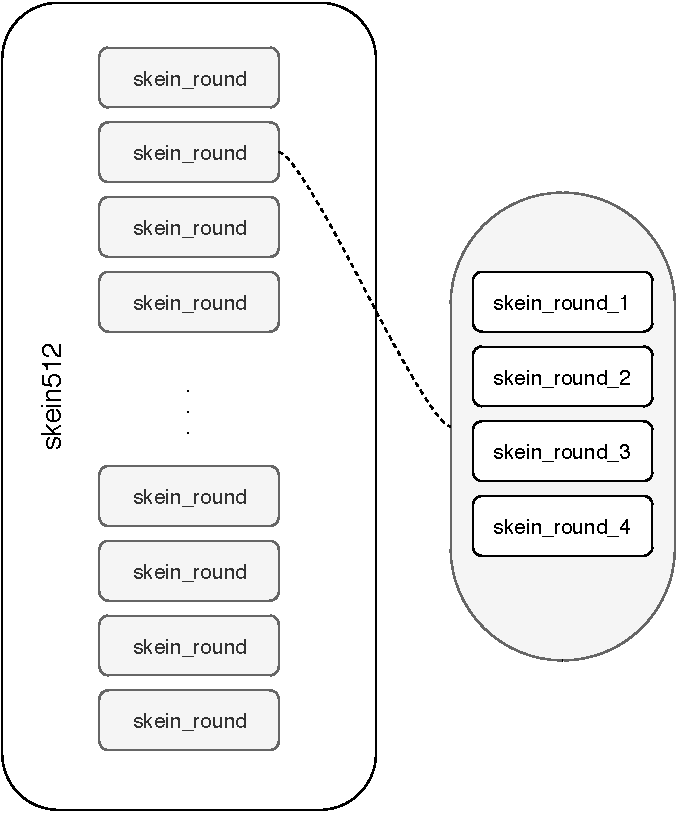
\includegraphics[width=10cm]{Images/VerilogDocumentation/modules_hierarchy.pdf}	
 	\caption{
 		نموداری از ساختار درختی و روابط ماژول ها با یکدیگر در طراحی
 	}
 \end{figure}
\section{
شبیه‌سازی
}
در مراحل طراحی قطعات سخت‌افزاری، پیش از تولید نهایی قطعات، به کمک نرم‌افزار‌های شبیه‌ساز، طراحی انجام شده شبیه‌سازی می شود. برای انجام شبیه‌سازی لازم است نحوه ی ورودی و خروجی گرفتن از طراحی، مشخص شود. این‌کار به کمک طراحی جداگانه‌ای به نامِ
\textit{\lr{Test Bench}}
صورت می‌گیرد. ما برای شبیه‌سازی از یک تست بنچ تغیر یافته از همان تست‌بنچ پیشنهادی استفاده کردیم ( 
\href{https://github.com/VahidZee/SkeinHashingHDL/blob/master/SourceCode/Verilog/testbench.v}
{
	این فایل
} 
)
مدت زمان شبیه‌سازی در این تست‌بنچ ۱۵۰۰۰ نانو ثانیه (۱۵۰۰ کلاک) درنظر گرفته شده است. برای شبیه‌سازی از نرم‌افزار 
\textit{\lr{ModelSim}}
استفاده شده است.
\subsection{توضیح تست‌بنچ}
تست‌بنچ طراحی شده ابتدا ورودی‌های صفر به قطعه‌ی
\lr{skein512}
می‌دهد، پس از ۵۰۰۰ نانو ثانیه یک‌سری ورودی و دوباره پس از ۵۰۰۰ ‌نانو ثانیه یک‌سری ورودی دیگر به قطعه می‌دهد. از نتایجی که این شبیه‌سازی به ما می‌دهد، میزان زمانی است که طول می‌کشد تا خروجی مناسب توسط قطعه تولید شود، دیگر آن‌که خود خروجی داده شده معرف درستی یا نا‌درستی طراحی انجام شده است.


\subsection{نتایج شبیه‌سازی}
نتایج کلی این شبیه‌سازی در تصاویر زیر قابل مشاهده‌اند:
\begin{figure}[H]
	\centering
	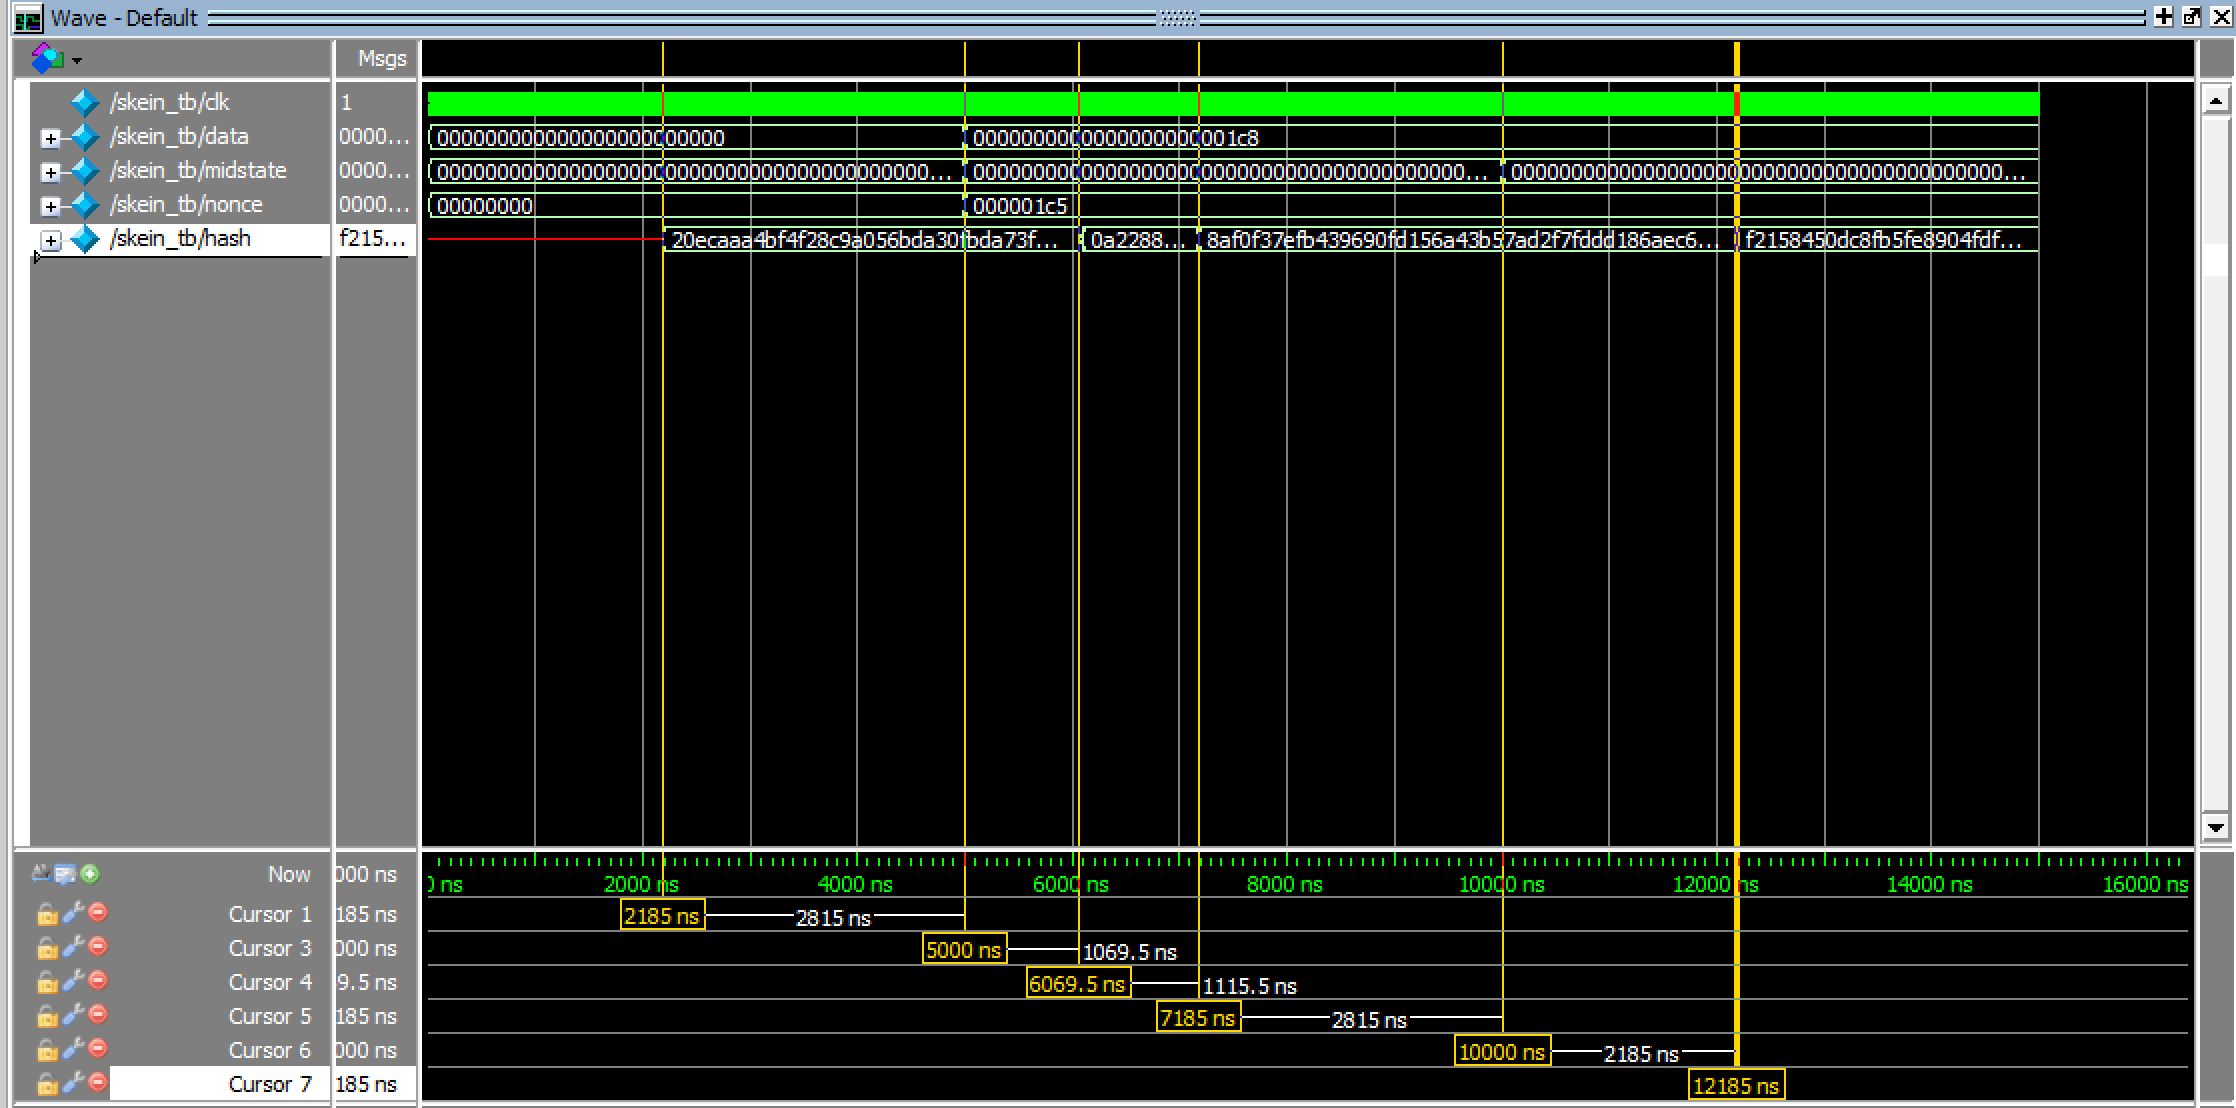
\includegraphics[width=16cm]{../RunData/sim_whole.png}	
	\caption{
	شکل موج مربوط به کل زمان شبیه‌سازی همراه با زمان‌های مهم
	}
\end{figure}
همان‌طور که مشخص است، هر‌بار که ورودی قطعه تغیر می‌کند، تقریبا ۲۸۱۵ نانو ثانیه طول می‌کشد که خروجی قطعه به حالت پایدار و نهایی خود برسد و قبل از این زمان خروجی قطعه ممکن است چندباری تغیر کند و مقدار درهم‌سازی نهایی نباشد، بنابر‌این در عمل این قطعه پس از
\textbf{ ۲۱۸ پالس ساعت }
جواب تولید خواهد کرد و درواقع ۲۱۸ پالس ساعت تاخیر دارد.

علت این مقدار تاخیر کاملا واضح است، طراحی انجام شده شامل ۷۲ 
\lr{round}
بوده و هر یک از این 
\lr{round}
ها دقیقا پس از ۴ کلاک خروجی خود را به بلاک بعدی انتقال می‌دهند. بنابر‌این
 $72 \times 4 = 218$ 
 کلاک طول خواهد کشید که جواب نهایی قطعه تولید شود، که این همان مقدار تاخیر مشاهده‌شده در شبیه‌سازی است.

\begin{figure}[H]
	\centering
	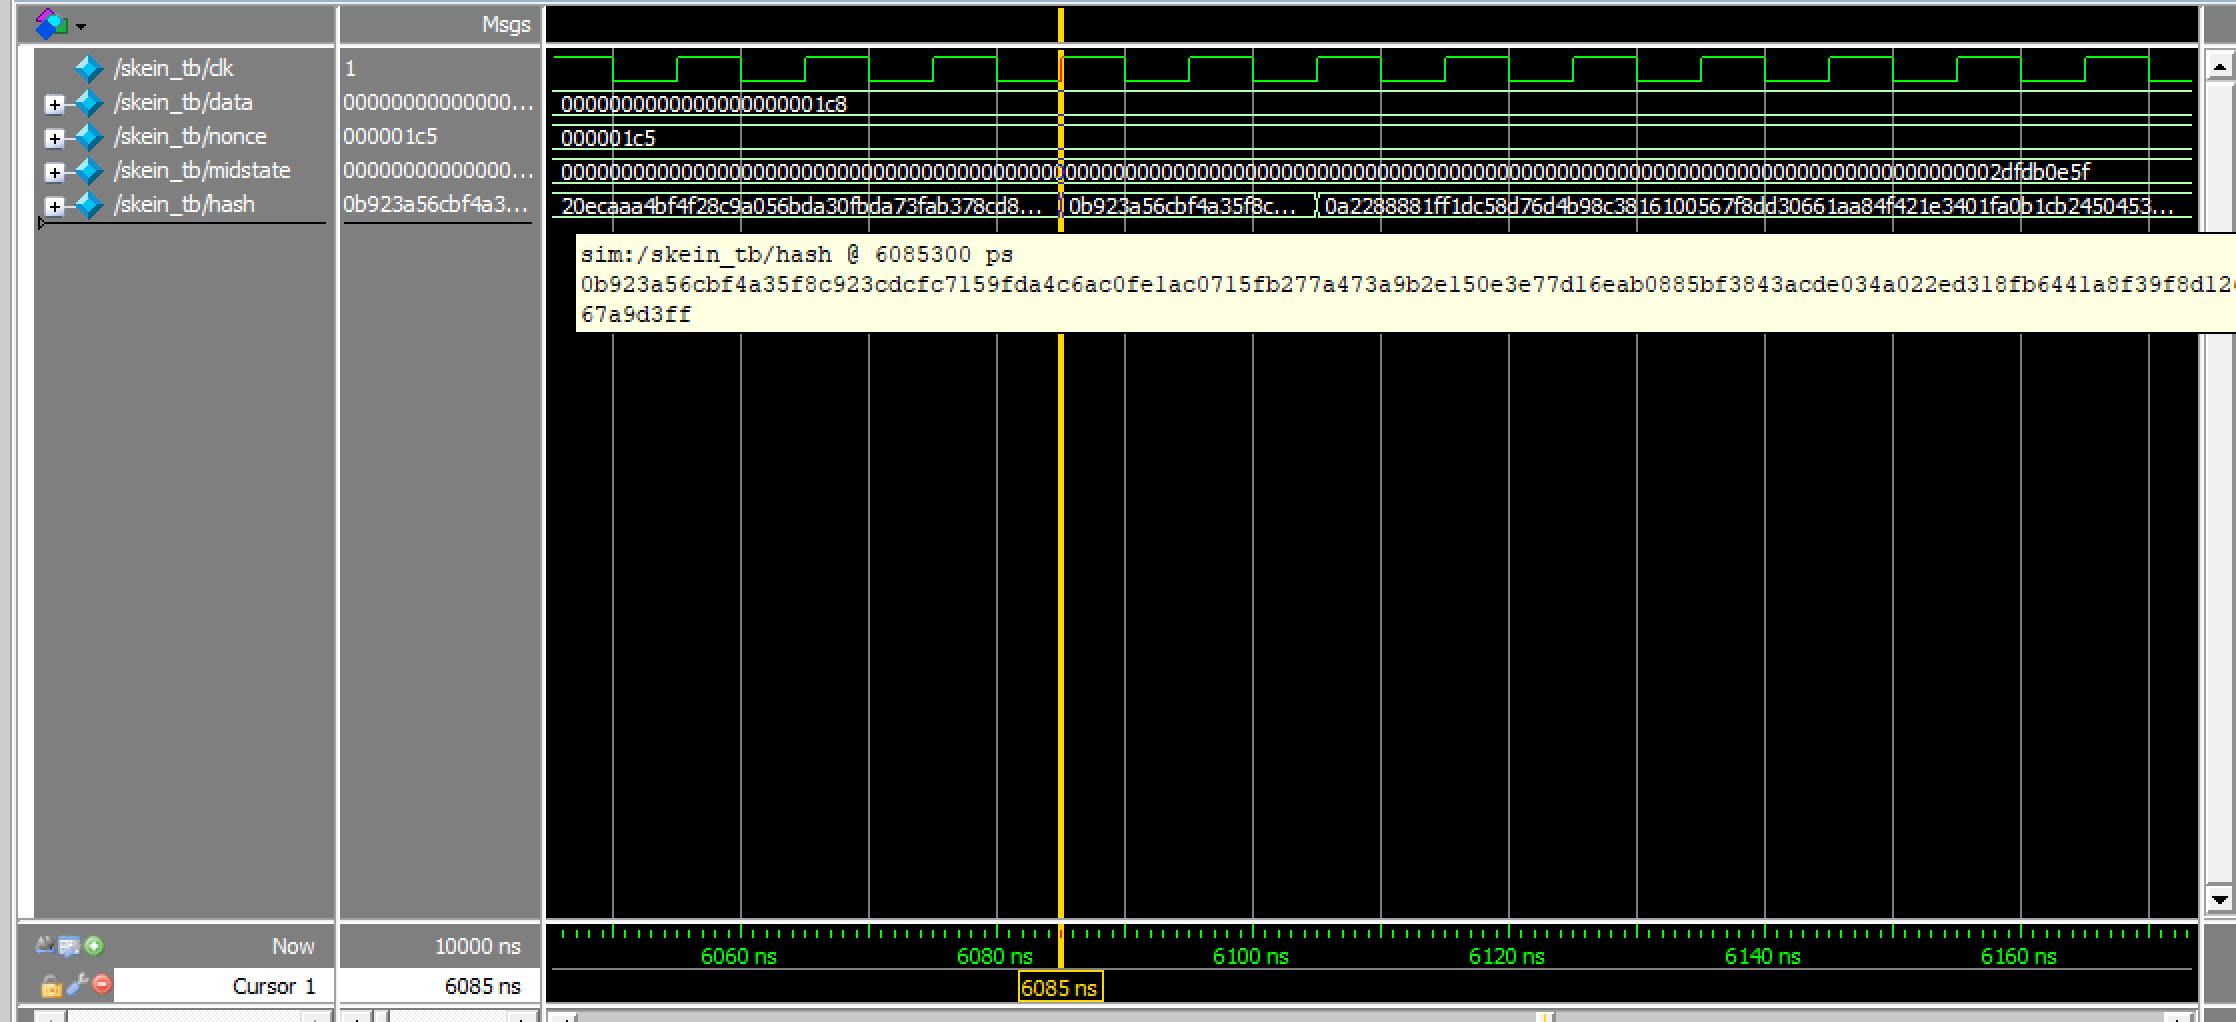
\includegraphics[width=16cm]{../RunData/sim_glitch1.png}	
	\caption{
		تولید خروجی غلط پیش از گذشت زمان ۲۱۸ پالس ساعت از لحظه‌ی تغیر ورودی
	}
\end{figure}
\begin{figure}[H]
	\centering
	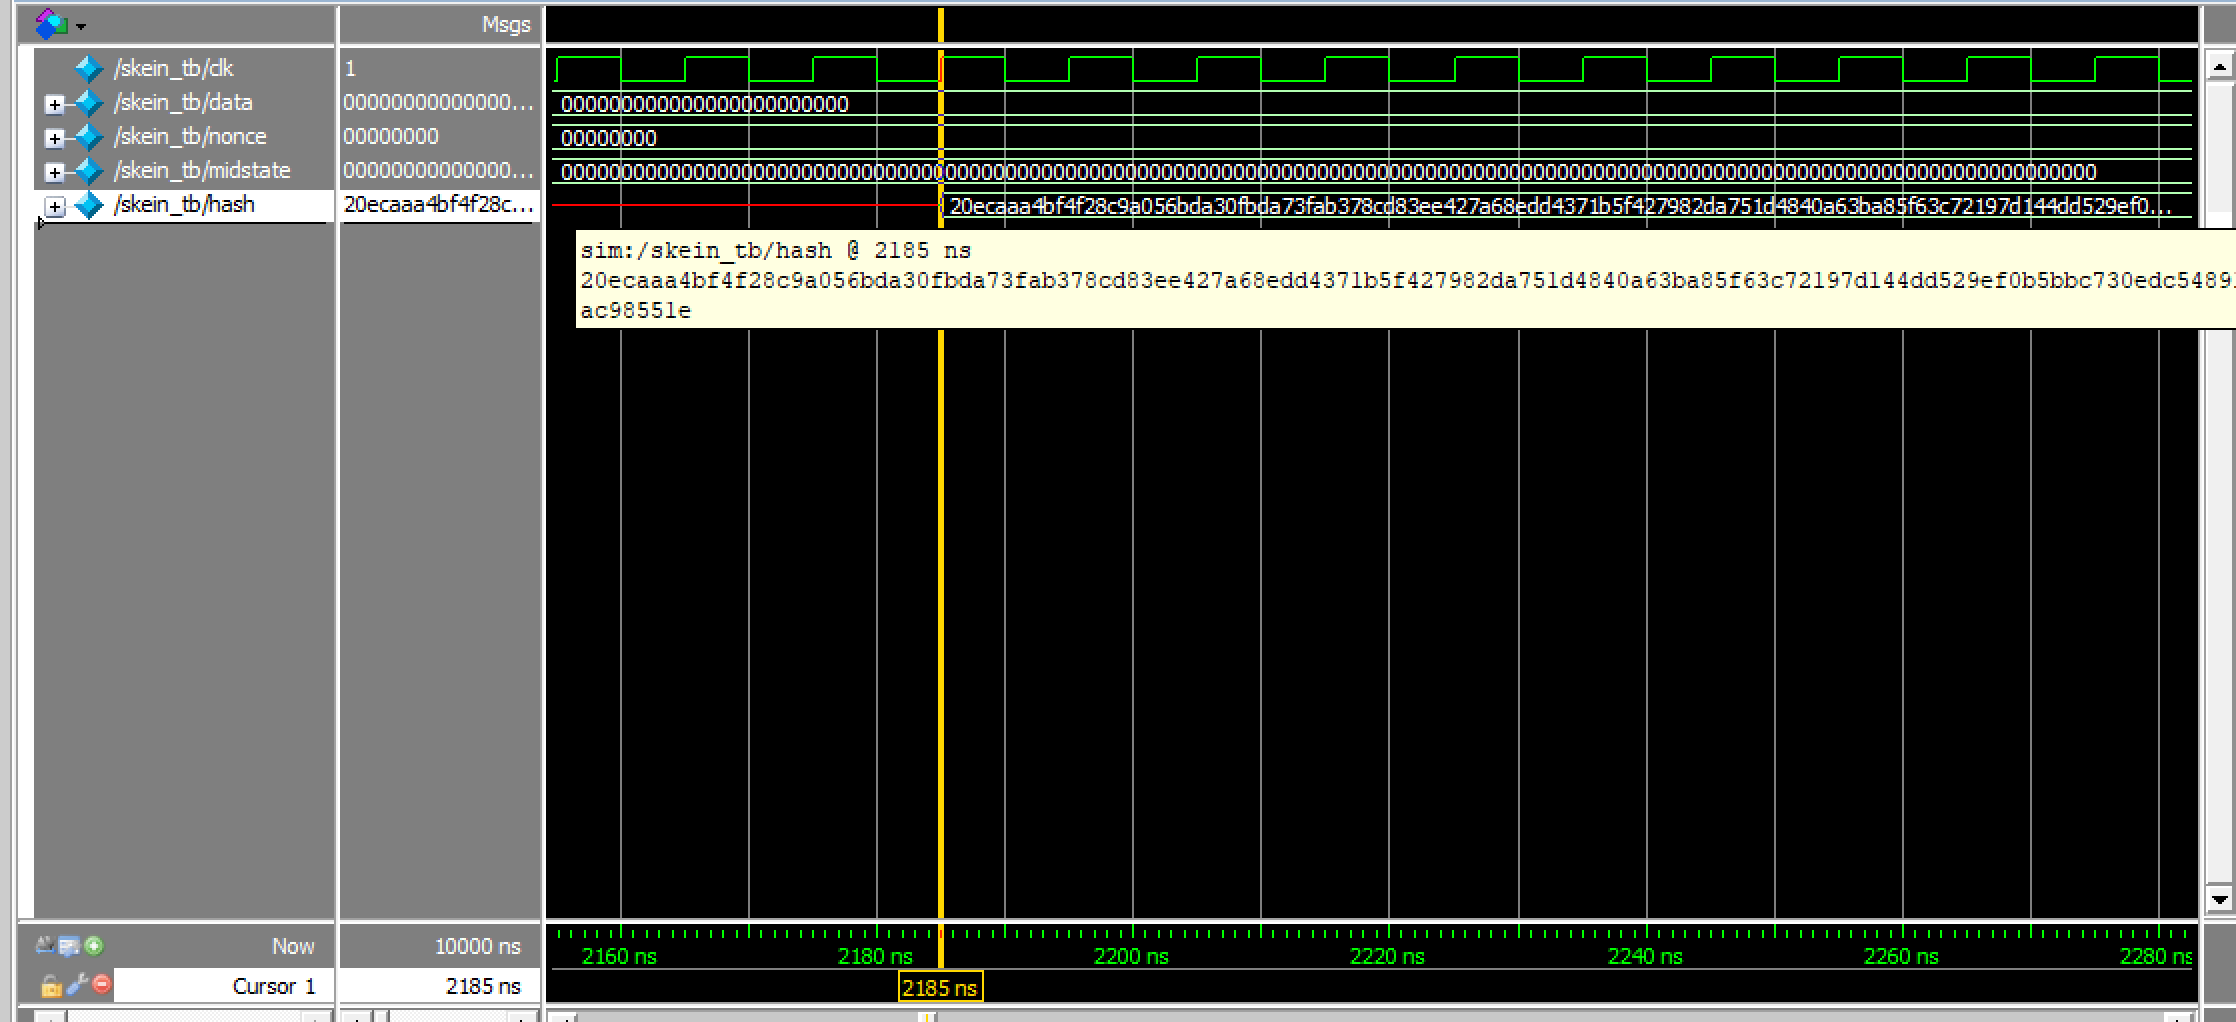
\includegraphics[width=16cm]{../RunData/sim_part1.png}	
	\caption{
		پاسخ تولید شده برای ورودی‌های صفر، پس از گذشت ۲۱۸ پالس ساعت
	}
\end{figure}
\begin{figure}[H]
	\centering
	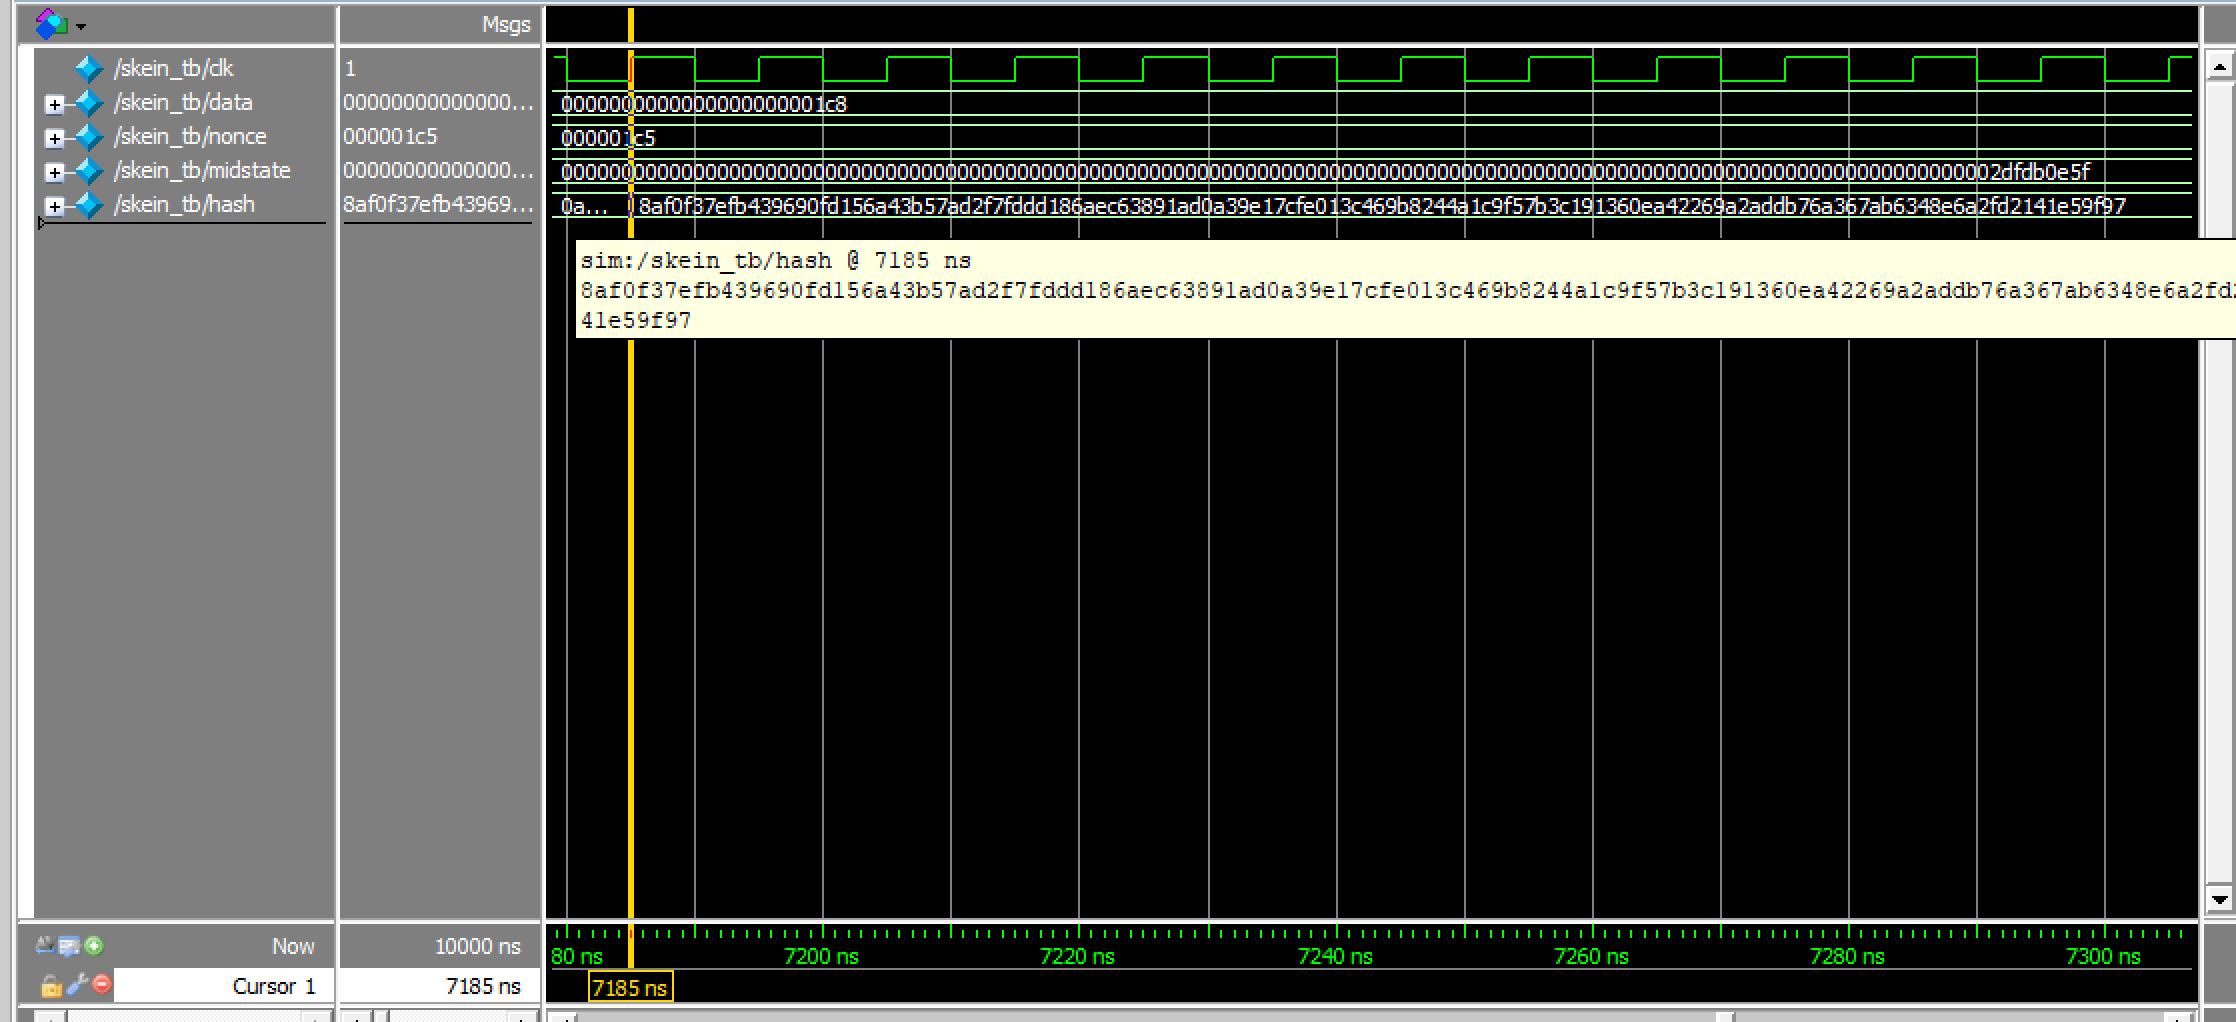
\includegraphics[width=16cm]{../RunData/sim_part2.png}	
	\caption{
		پاسخ تولید شده برای ورودی‌های داده شده پس از ۵۰۰۰ نانو ثانیه، پس از گذشت ۲۱۸ پالس ساعت
	}
\end{figure}
\begin{figure}[H]
	\centering
	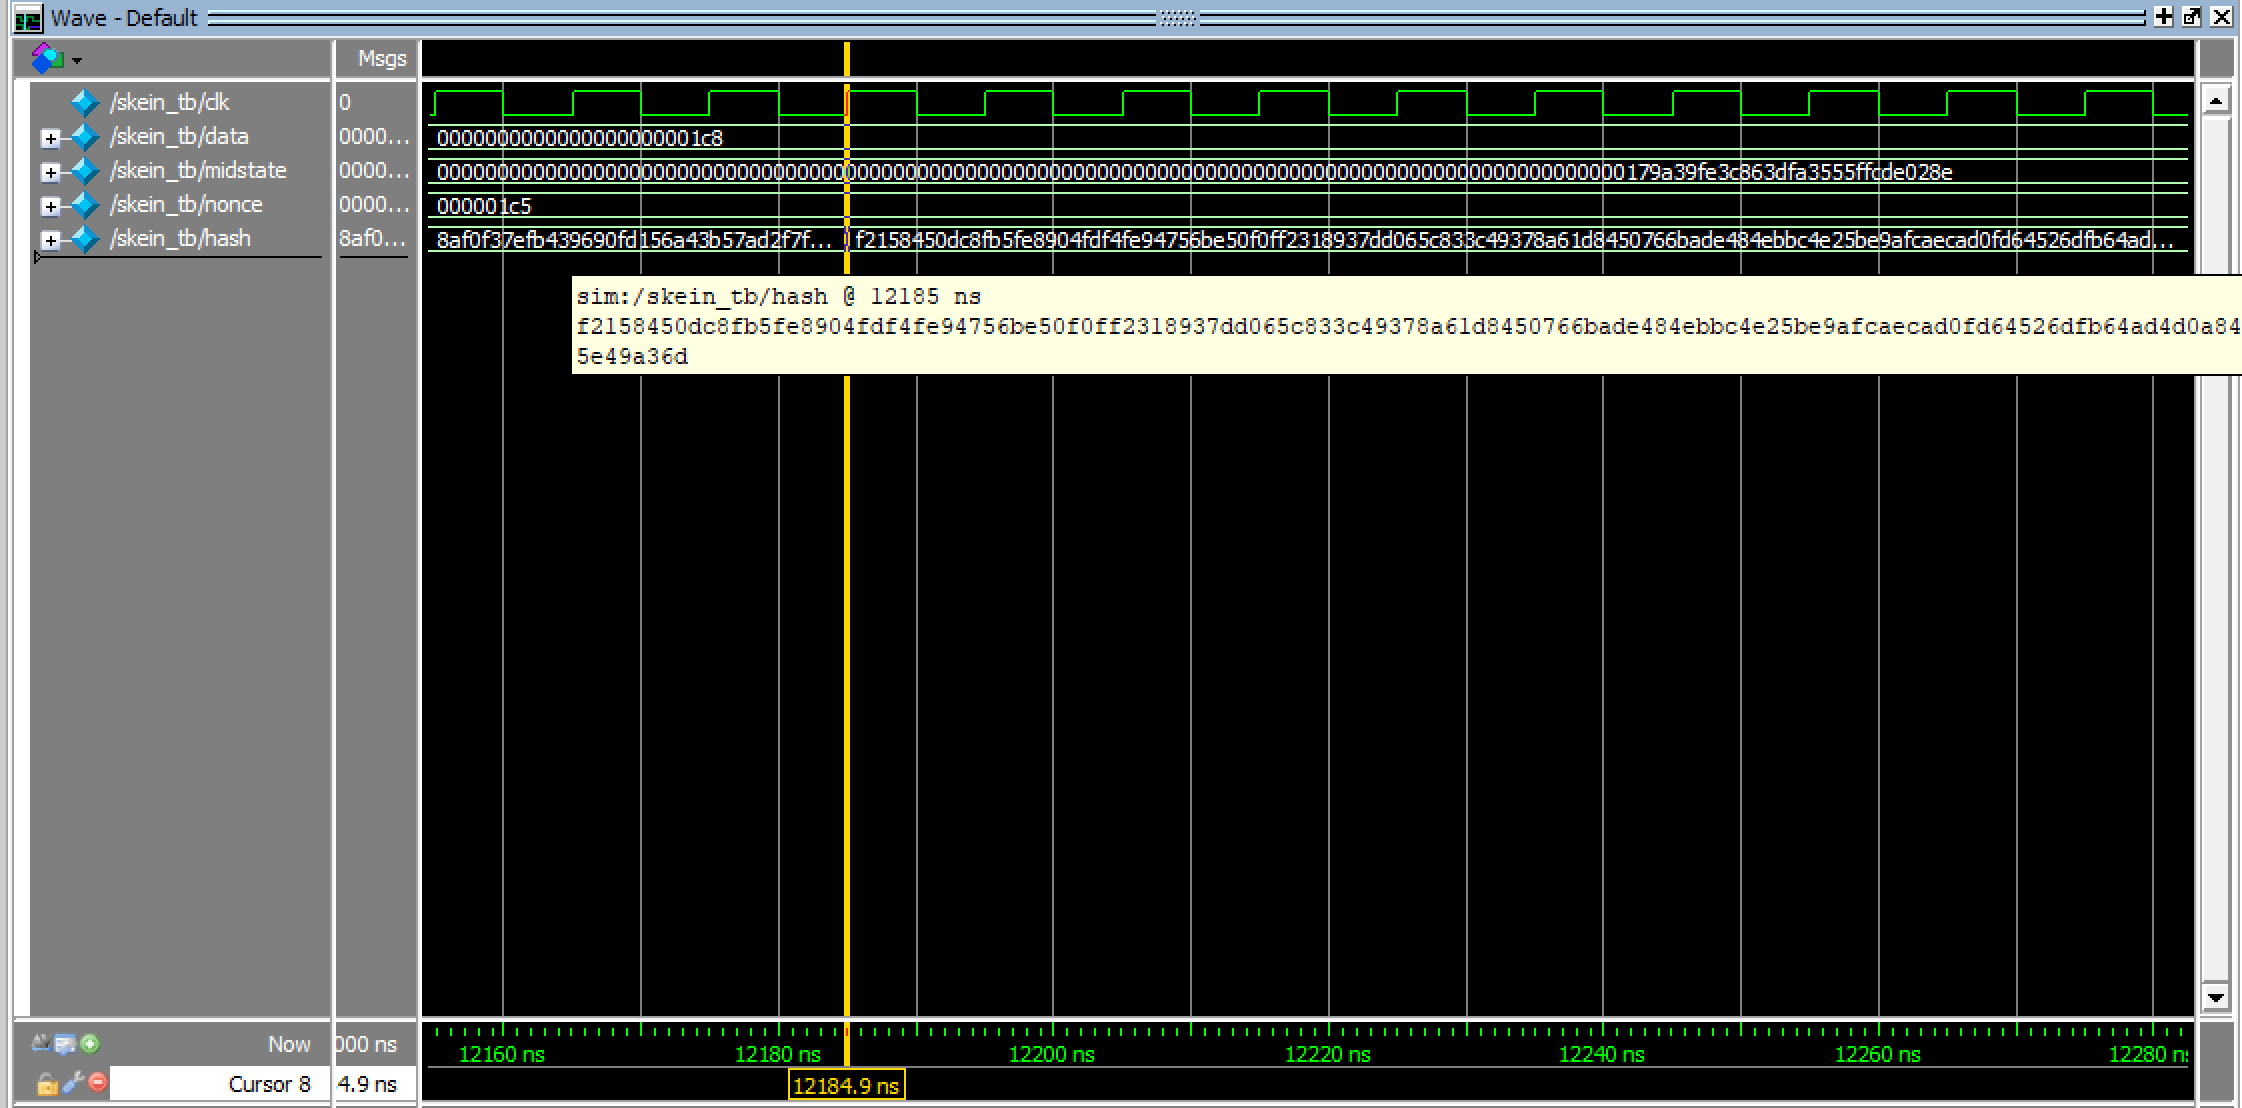
\includegraphics[width=16cm]{../RunData/sim_part3.png}	
	\caption{
		پاسخ تولید شده برای ورودی‌های داده شده پس از ۱۰۰۰۰ نانو ثانیه، پس از گذشت ۲۱۸ پالس ساعت
	}
\end{figure}

	\chapter{مدل طلایی}
\label{chapter:GoldenModel}
\section{مقدمه}
در مدل‌ طلایی ۴ نوع متفاوت از \lr{Skein hash} آورده شده‌است (‌ ۲۲۴ و ۲۵۶ و ۳۸۴ و ۵۱۲  بیت) که همانطور که در مدل  طراحی شده با \lr{verilog} نیز تنها نوع استاندارد  (۵۱۲ بیت)آن پیاده‌سازی شده است , در مدل‌ طلایی نیز تنها توضیحات و مستندات این نوع ارائه خواهد شد.
\\
\begin{center}
	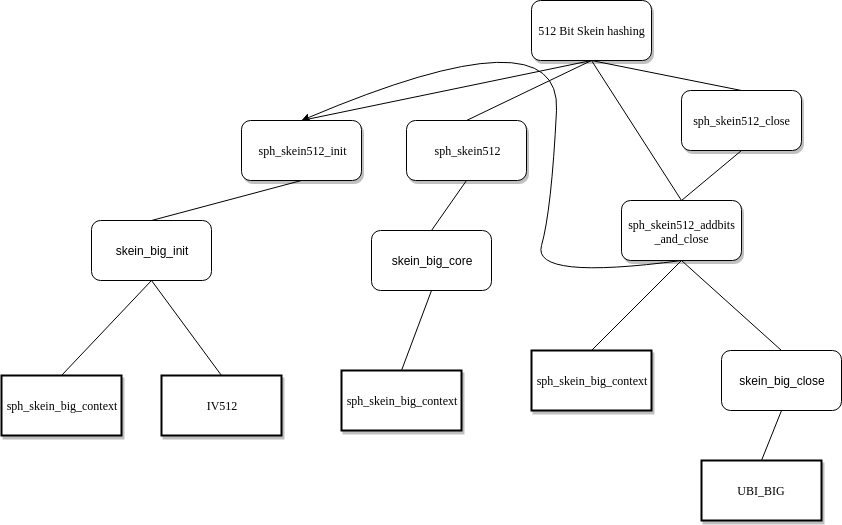
\includegraphics[width=16cm]{images/GoldenModel.png}
\end{center}

\section{پیاده‌سازی الگوریتم}
در شکل بالا تمامی توابع و ساختارهای مورد نیاز  و سلسله مراتب آن‌ها برای نوع ۵۱۲ بیتی الگوریتم آورده شده است , برای توضیح نحوه‌ی اجرای الگوریتم با شروع از  
\lr{sph-skein-big-context} سلسله اجرای برنامه توضیح داده خواهد شد.
\\
در این برنامه برای ‌ذخیره و استفاده از هش , از ساختاری استفاده شده است به نام \hyperref[subsec:sph-skein-big-context]{\lr{sph-skein-big-context}} استفاده شده است و هدف برنامه اجرای الگوریتم هش و ذخیره‌ی خروجی در این ساختاو بدست آوردن درهم‌سازی مورد نظر است.
\\
برای اجرای الگوریتم هش ۵۱۲ بیتی , در سلسله‌ی اجرا از توابع زیر استفاده شده است :
\\
در ابتدا برنامه با ذخیره‌ی مقادیر از پیش تعیین شده  \hyperref[subsec:IV512]{\lr{IV512}} در ساختار معرفی شده شروع به کار می‌کند , و این کار توسط تابع
\hyperref[subsec:sph-skein512-init]{\lr{sph-skein512-init}}
   انجام میگردد.
  \\ سپس با در نظر گرفتن ورودی و سایز این ورودی، اجرای الگوریتم هش  توسط تابع \hyperref[subsec:sph-skein512]{\lr{sph-skein512}}
   شروع می‌شود و ورودی داده شده تبدیل به هش میشود و با ذخیره شدن در ساختار  هش، این تابع پایان می‌پذیرد.
  \\ 
  حال برای فهم درست از توابع مورد استفاده لازم است نحوه‌ی پیاده‌سازی \hyperref[subsec:UBI-BIG]{\lr{UBI-BIG}} توضیح داده‌شود. تمامی سلسله مراتب طراحی آن در شکل زیر آورده شده‌است.
  \begin{center}
  		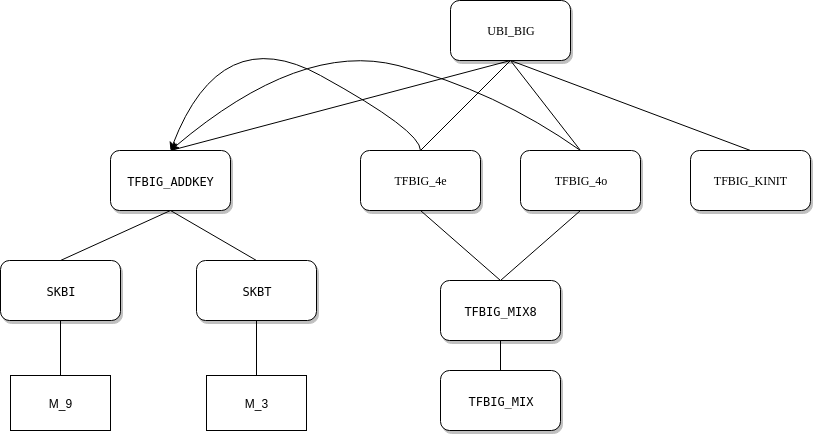
\includegraphics[width=16cm]{images/UBI.png}	
  \end{center}
%todo sajflashfkashfkjash
  
یه توضیح عه کوچیک برااا یو بی آی بیگ   ppppppppppppppppppppppppppppppp


	
	\section{ \textbf{ساختارها}}

\subsection{\lr{sph-skein-big-context}}
\label{subsec:sph-skein-big-context}
این ساختار مورد نظر برای ذخیره و استفاده از هش است (‌ شامل مقادیری از هش قبلی و مقادیر جدید محاسبه شده ). \\ این ساختار شامل یک آرایه‌ی ۶۴ بیتی از کاراکترهاست که به منظور تراز کردن انواع هش استفاده می‌گردد و  هشت عدد ۶۴ بیتی  که برای ذخیره‌ی ۵۱۲ بیت هش  استفاده می‌شوند  و هم‌چنین شامل دو عدد با نام‌های \lr{ptr, bcount} است که این دو عدد به طور معمول برابر ۰ هستند که همانند \lr{nonce} در پیاده‌سازی وریلاگ آن است.



\subsection{\lr{IV512}}
\label{subsec:IV512}
این ساختار شامل مقادیر اولیه‌ی هش است. یک عدد ۵۱۲ بیتی را برای خوانا بودن در مبنای ۱۶ و در ۸ بلاک ۱۶ بیتی نگاه می‌دارد. این مقدار در برنامه‌ به زبان وریلاگ همان \lr{midstate} است.
\subsection{\lr{UBI-BIG}}
\label{subsec:UBI-BIG}

در این تابع روی دیتای ذخیره شده در بافر عملیات درهم‌سازی انجام شده‌است. این درهم‌سازی برمبنای مقادیر قبلی موجود در $  h_0 $ تا  $ h_7 $ ( که در سری قبلی صدا شدن این تابع مشخص شده‌اند)، دیتا و ورودی‌های \lr{extra} و  \lr{etype} انجام شده‌است. 
در ابتدا سه\lr{ sph-u64 }با اسامی $ t_0 , t_1 , t_2 $ تعریف شده‌اند. \lr{ sph-u64 }جنسی تعریف شده برای متغیرهای ۶۴ بیتی بدون علامت است. سپس متغیری به اسم $ u $ تعریف شده‌ که در ادامه‌ی تابع به عنوان شمارنده در حلقه‌ها استفاده شده‌است. با شروع از \lr{buf} هر هشت عنصر که هر کدام یک بایت هستند توسط \lr{sph-dec64le-aligned} به ۶۴ بیت پشت سر هم تبدیل شده و سپس به$ m_0 $تا $ m_7 $ داده شده‌اند.  \lr{sph-dec64le-aligned} یک بیت به عنوان شروع هشت بایت ورودی گرفته سپس هشت بایت را به یک دیکودر داده و ۶۴ بیت خروجی می‌دهد. مقدارهای $ m_0 $ تا $ m_7 $ در $ p_0 $ تا $ p_7 $ ریخته شده‌اند. $ m_0 $ تا $ m_7 $ تا اخر تابع بدون تغییر باقی مانده و مقدارهای اولیه‌ی بخش‌های دیتا هستند.  
سپس مقدار ‌\lr{extra} پس از \lr{cast} به\lr{sph-u64} با مقدار \lr{bcount} با ۶ بیت شیفت به چپ جمع شده و به $ t_0 $ داده شده‌است. سپس مقدار ‌\lr{bcount} ، ۵۸ بیت به راست شیفت داده شده و ‌\lr{etype} هم ۵۵ بیت به چپ شیف داده شده‌است. این مقادیر با هم جمع شده‌‌اند و جمعشان به ‌$ t_1 $ داده شده‌است. مقدار شیفت داده شدن‌ها از روی شکل زیر قابل توجیه‌اند:
\begin{center}
	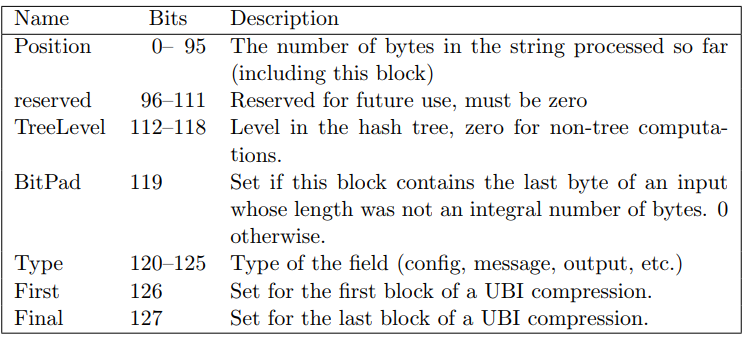
\includegraphics[width=14cm]{Images/GoldenModelDocumentation/tweak.png}
\end{center}

در این جدول \lr{TreeLevel} همان \lr{bcount} است که در تابع\hyperref[subsec:skein-big-core]{\lr{skein-big-core}} در هربار صدا کردن \lr{UBI-BIG} مقدار آن یک واحد افزوده می‌شود. \lr{etype} برای رد کردن بخش \lr{position} و هم‌چنین مشخص کردن بیت \lr{first}  است و \lr{extra} برای تعیین بیت \lr{final} و \lr{bitpad} استفاده شده‌است. پنج بیت خالی هم برای \lr{Type}قرار داده شده و هم‌چنین بخش \lr{reserved} هم صفر هست. 
\\
سپس تابع\hyperref[subsec:TFBIG-KINIT]{\lr{TFBIG-KINIT}}
صدا شده تا مقدار $ t_2 $ و $ h_8 $ برمبنای بقیه ورودی های تابع یعنی $ t_1 , t_0 $ و $ h_0 $ تا $ h_7 $ تعیین شوند. سپس برای اعداد زوج بین ۰ تا ۱۷\hyperref[subsec:TFBIG-4e]{\lr{TFBIG-4e}} و برای فردها \hyperref[subsec:TFBIG-4o]{\lr{TFBIG-4o}} صدا شده‌اند. به این ترتیب میکس در ۱۸ سری چهار تایی اجرا شده که هر کدام ۴ \lr{round} دارند و هر ۸ سری صدا شدن یکی‌است و در هر یک از این ۱۸ سری دانستن زوج و فرد بودن سری کافیست. هم‌چنین هر چهار بار یعنی در ابتدای هر \lr{TFBIG-4e}یا\lr{TFBIG-4o} یک بار\hyperref[subsec:TFBIG-ADDKEY]{\lr{TFBIG-ADDKEY}}صدا شده تا بر مبنای شماره‌ی سری که در این‌جا با $ s$ نمایش داده شده و همین‌طور $ i $در $ pi $ و باقی مانده گرفتن از جمعشان کلید جدید مشخص شده و با \lr{pi} جمع شود. این‌جا از$ h_0 $تا$ h_7 $که حاصل سری قبلی اجرای\lr{UBI-BIG} است و همین‌طور \lr{tweak} ها استفاده شده تا مقدار جدید $ pi $ تعیین و در سری بعد استفاده شود. سپس برای بار هجدهم \lr{TFBIG-ADDKEY} صدا شده‌است. در نهایت $ hi $ از $ xor $ گرفتن $pi $ و $ mi $ به دست ‌آمده‌است. پس ‌‌‌$ hi $ نشان‌دهنده‌ی بیت‌های تغییر یافته‌ی ‌$ pi $ در طول تابع است.


\subsection{\lr{TFBIG-4e}و \lr{TFBIG-4o}}
\label{subsec:TFBIG-4e}
\label{subsec:TFBIG-4o}

این تابع برای کدگذاری $ P_0 $ تا $ P_7 $ طراحی شده‌است. همان‌طور که پیش‌تر توضیح داده شده است، ۷۲ بار تابع درهم‌سازی صدا می‌شود،‌ و هر ۸ سلسله از این ۷۲ مرحله یکسان است، هم‌چنین در هر ۸ سری ۴ بار با یک کلید و ۴ بار دیگر با یک کلید دیگر اجرا می‌شود،‌ که به همین دلیل این توابع  هر کدام برای آن ۴ باری استفاده می‌شود که در مرحله‌ای زوج یا فرد قرار داریم.
\\
این تابع یک ورودی  \lr{s} دارد. تابع  \hyperref[subsec:TFBIG-ADDKEY]{\lr{TFBIG-ADDKEY }} با ‌$ p_0 $ تا  $ p_7 $ و $ h $ و $ t $و ‌$ s $ به ترتیب به عنوان  $ w_0 $ تا $ w_7 $و $ k $و ‌$ t $ و ‌$ s $ صدا شده‌است. ‌$ h $ و $ t $ برای \lr{concat} و ساختن کلید در تابع 
\lr{TFBIG-ADDKEY}
 استفاده شده‌اند.
سپس   
\hyperref[subsec:TFBIG-MIX8]{\lr{TFBIG-MIX8 }}`
چهار بار برای ترتیب‌های متفاوتی از ‌$ p_0 $ تا $ p_7 $ اعداد متفاوت به عنوان $ rc $ صدا شده‌است. ترتیب صدا شدن $ p_0 $ تا $ p_7 $ برای تعداد بلاک ۸ به صورت جدول‌های زیر است،‌ که برای هر ‌‌راند از ۰ تا ۳، بر حسب راند قبل ترتیب‌ها چهار عدد جابه‌جا شده‌اند. و تفاوت حالت‌های زوج و فرد در اعداد استفاده شده است. در جدول‌ها 
\lr{N\_w} تعداد 
\lr{cypher block}هاست که در این کد ۸ است. همین‌طور \lr{j} همان شماره‌‌ی راند در ماژول‌های وریلاگ است.
\begin{center}
	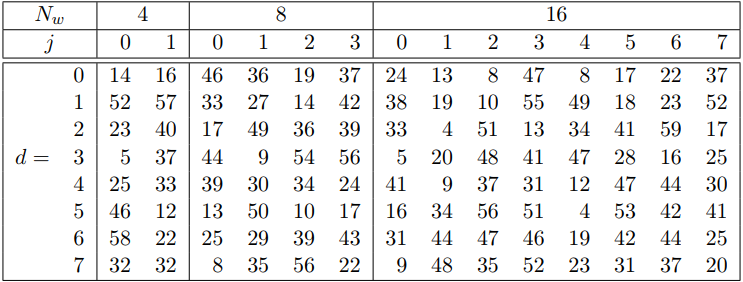
\includegraphics[width=10cm]{Images/GoldenModelDocumentation/table_mix.png}
	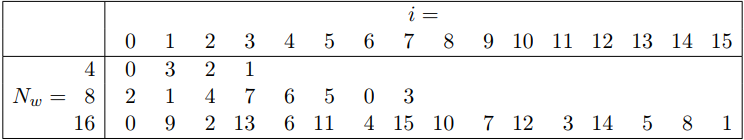
\includegraphics[width= 10cm]{Images/GoldenModelDocumentation/Mix2.png}
\end{center}


\subsection{\lr{TFBIG-ADDKEY}}
\label{subsec:TFBIG-ADDKEY}

این تابع طبق فرمول‌های زیر مقادیر ورودی را تغییر می‌دهد و برای اینکار از تابع‌های \hyperref[subsec:SKBI]{\lr{SKBI}} و \hyperref[subsec:SKBT]{\lr{SKBT}} استفاده می‌کند که به ترتیب جمع مقادیر ورودی‌شان را به پیمانه ۳ و ۹ محاسبه می‌کنند.
\\متغیرهای $ h_0 $ تا $ h_8 $ در تولید کلید استفاده می‌شوند، برای محاسبه‌ی اندیس آن‌ها ( از ۰ تا ۸ ) از \lr{SKBI} استفاده شده است.
\\
متغیر‌های دیگری که در تولید کلید استفاده شده‌اند $ t_0 $ تا $ t_2 $ هستند که برای تولید اندیس آن‌ها از تابع \lr{SKBT} استفاده شده است.\\
\begin{latin}
	\begin{center}
		\begin{tabular}{c c}
			$k_{s, i} = k_{(s+i) \mod 9} $ \hspace{15mm} & $  i = 0, 1, 2, ... , 4 $ \\
			
			
		\end{tabular}
		\\
		$k_{s, 5} = k_{(s+5) \mod 9} + t_{s \mod 3}$ \\
		$k_{s, 6} = k_{(s+6) \mod 9} + t_{(s+1) \mod 3}$ \\
		$k_{s, 7} = k_{(s+7) \mod 9} + s $\\	
	\end{center}
\end{latin}

دقت شود که تمامی این محاسبات برای نوع ۵۱۲ بیتی الگوریتم است.




\subsection{\lr{SKBI}}
\label{subsec:SKBI}

تابع \lr{SKBI} برای محاسبه‌ی اندیس کلید استفاده‌ شده‌است. \\ 
در الگوریتم برای تولید $k_0 $ تا $ k_8 $ از این ماکرو استفاده شده ‌است.  ,این ماکرو $ k $ و $ s $ و $ i $ را گرفته و سپس $ k $ را به \lr{ M9-s-i }متصل می‌شود که باقی‌مانده‌ی ‌$s + i $بر ۹ تعریف شده‌است.


\subsection{\lr{SKBT}}
\label{subsec:SKBT}
برای تولید $ t_0 $ تا $ t_2 $ از این ماکرو استفاده شده است، $ t $ و $ s $ و ‌$ i $ به این تابع داده شده و سپس $ t $ به \lr{M3-s-i} متصل شده است که باقی‌مانده‌ی $ s + i $ بر ۳ تعریف شده است.

\subsection{\lr{TFBIG-MIX8}}
\label{subsec:TFBIG-MIX8}


همان‌طور که در مقدمه گفته‌ شده‌است،‌ هر سری از هشت سری، چهار \lr{round} دارد، پس طراحی این تابع برای ساده‌سازی استفاده‌ی متداول از \hyperref[subsec:TFBIG-MIX]{\lr{TFBIG-MIX}} بوده‌است. به صورت متداول در کد به چهار سری استفاده از  \lr{TFBIG-MIX}پشت سر هم نیاز است. 


\subsection{\lr{TFBIG-MIX}}
\label{subsec:TFBIG-MIX}

وظیفه‌ی این تابع درهم سازی بلاک‌های ورودی طبق فرمول‌های زیر است.
\begin{center}
	$y_0 = (x_0 + x_1) \mod 2^{64}$ \\
	$ y_1 = (x_1 <<< R_{(d \mod 8), j}) \oplus y_0$
\end{center}
که مقادیر $ R $ در جدول زیر آمده است :

\begin{center}
	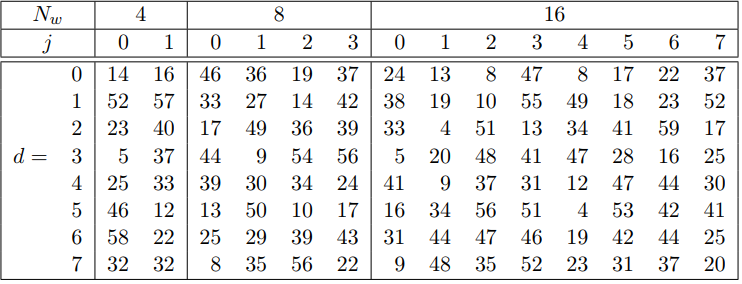
\includegraphics[width=10cm]{Images/GoldenModelDocumentation/MIX1.png}
\end{center}




\subsection{\lr{TFBIG-KINIT}}
\label{subsec:TFBIG-KINIT}
این تابع با ورودی‌های $ t_0 $ تا $ t_2 $ و $h_0 $ تا $ h_8 $ مقادیر زیر را محاسبه می‌کند :
$$
k_8 = C \oplus k_0 \oplus k_1 \oplus ... \oplus k_7
$$

$$
t_2 = t_1 \oplus t_0
$$
که مقدار ثابت $ C $ به آن جهت در فرمول وجود دارد که از ۰ نبودن تمامی بیت‌ها اطمینان حاصل شود.

\subsection{\lr{DECL-STATE-BIG}} 
\label{subsec:DECL-STATE-BIG}


در این ماکرو متغیرهای ‌$ h_0 $ تا $ h_7 $ و \lr{bcount} هر دو از جنس\lr{sph-u64} (متغیر ۶۴بیتی بدون علامت) تعریف شده‌اند. 


\subsection{\lr{READ-STATE-BIG}} 
\label{subsec:READ-STATE-BIG}


این تابع برای خواندن اطلاعات از ورودی و ذخیره‌ی ‌‌آن‌ها بر روی متغیرهاست به طور دقیق‌تر  به این تابع ‌بلاک \lr{sc} به عنوان ورودی داده شده‌است. در آن متغیرهای $ h_0 $ تا $ h_7 $ و \lr{bcount} استراکت به ترتیب به متغیرهای ‌$ h_0 $ تا $ h_7 $ و \lr{bcount} کد مقداردهی شده‌اند.

\subsection{\lr{WRITE-STATE-BIG}} 
\label{subsec:WRITE-STATE-BIG}


این تابع برای ذخیره‌ی اطلاعات بر روی \lr{struct} است.\\
به این تابع ورودی \lr{struct}  با نام \lr{sc} داده شده‌است. متغیرهای $ h_0 $ تا $ h_7 $ و همین‌طور \lr{bcount} کد، در $ h_0 $  تا  $ h_ 7 $ و \lr{bcount}  ساختار
ذخیره شده‌اند.

\section{ توابع}

\subsection{\lr{sph-skein512-init}}
\label{subsec:sph-skein512-init}
این تابع مسئولیت مقداردهی اولیه‌ی ساختار هش را بر عهده دارد، که برای آن تابع \hyperref[subsec:skein-big-init]{\lr{skein-big-init}} را با ورودی‌ اولیه‌ی \lr{IV512} اجرا می‌کند.
\subsection{\lr{skein-big-init}}
\label{subsec:skein-big-init}

این تابع دو ورودی می‌پذیرد که یکی از آن‌ها آدرس یک ساختار هش است و دیگری مقدار اولیه، که مقادیر متناظر ساختار داده شده را برابر مقادیر اولیه قرار می‌دهد.
که مقدار اولیه در حالت ۵۱۲ بیتی در ساختار \lr{IV512} ذخیره شده ‌است.

\subsection{\lr{sph-skein512}}
\label{subsec:sph-skein512}

در این تابع ماکروی\hyperref[subsec:skein-big-core]{\lr{skein-big-core}} صدا شده‌است. ورودی‌های این تابع که بدون انجام هیچ پردازشی به \hyperref[subsec:skein-big-core]{\lr{skein-big-core}} پاس داده‌ شده‌اند،‌ ‌\lr{cc} که همان ساختار هش است، \lr{data} که داده‌ی ورودی است و ‌\lr{len} که طول  \lr{data} است، هستند.


\subsection{\lr{skein-big-core}}
\label{subsec:skein-big-core}

در این تابع  همه‌ی بلاک‌های دیتا به‌جز بلاک اخر در دسته‌های ۵۱۲ تایی هش شده‌اند. مقدار ‌\lr{bcount} هم برای استفاده‌ی ثانویه تعیین شده و هم‌چنین آخرین بلاک دیتا در بافر ریخته‌ شده‌است. \\


به این تابع ورودی‌های ‌\lr{sc} که  ساختار هش است، \lr{data} که داده‌ی ورودی برای هش است و \lr{len} که طول \lr{data} است پاس داده شده‌اند. در ابتدای تابع با صدا شدن \hyperref[subsec:DECL-STATE-BIG]{\lr{DECL-STATE-BIG}} متغیرهای لازم تعریف شده‌اند. سپس در یک $ if $ بررسی شده‌است که برای دیتا در بافر فضای کافی هست یا نیست: \\
- در صورتی که فضا باشد،‌ کل دیتا از جایی که پوینتر به آن اشاره کرده‌است دخیره شده‌ و سپس پوینتر که به پایان دیتای ذخیره شده اشاره دارد به اندازه‌ی طول دیتا به جلو جابه‌جا شده‌ و در خود ‌\lr{struct} هم مقدار ‌آن \lr{update} شده‌ و سپس از تابع خارج شده‌است.
\\
- در غیر این صورت، ابتدا  \hyperref[subsec:READ-STATE-BIG]{\lr{READ-STATE-BIG}} صدا شده‌است. متغیر \lr{first} یک متغیر هشت بیتی با هشت بیت ۰ یا یک بیت پرارزش یک و بقیه ۰ است. اگر این تابع به طور متدوال از\hyperref[subsec:skein-hash]{\lr{skein-hash}}صدا شود \lr{first} برابر با ۱۲۸ می‌شود. سپس در یک لوپ ابتدا در صورت پر بودن بافر از دیتا (به این معنی که پوینتر برابر با سایز بافر شده‌باشد)،‌ اول  \lr{bcount} یکی زیاد شده‌است. سپس\hyperref[subsec:UBI-BIG]{\lr{UBI-BIG}} برای $ first + 96 $ به عنوان \lr{etype} و ۰ به عنوان \lr{extra} صدا شده‌است. پس از آن \lr{first} و \lr{ptr} هر دو صفر گذاشته شده‌اند تا برای سری بعد پر شدن دیتا بافر از ابتدا \lr{overwrite} شود. سپس شرط پر بودن بافر تمام شده و به اندازه‌ی مینیموم مقداری که در بافر جا هست با طول دیتای باقی‌مانده در بافر دیتا ذخیره شده‌است. پوینتر و دیتا با مقدار این مینیموم جمع و \lr{len} منهای آن شده‌ تا مقدار دیتای باقی‌مانده را نشان دهد. و سپس حلقه تا زمانی که هنوز دیتایی باقی مانده‌باشد تکرار می‌شود. درواقع در این حلقه هر سری به تعداد بزرگترین مضرب سایز بافر که اکیدا کوچک‌تر از \lr{len} دیتا است تکرار شده و هر سری روی همان طول از دیتا \hyperref[subsec:UBI-BIG]{\lr{UBI-BIG}} صدا شده‌است. \lr{bcount} همین تعداد بار را نشان می‌دهد. برای آخرین سری که کوچک‌تر مساوی سایز بافر است، در بافر ذخیره شده و \lr{ptr} به آخر آن اشاره کرده‌است. 
در آخر \hyperref[subsec:WRITE-STATE-BIG]{\lr{WRITE-STATE-BIG}}
صدا و بعد مقدار فعلی پوینتر هم در \lr{struct} ذخیره شده‌است. 
نحوه ذخیره‌سازی \lr{tweak} به شکل زیر است. 
\begin{center}
	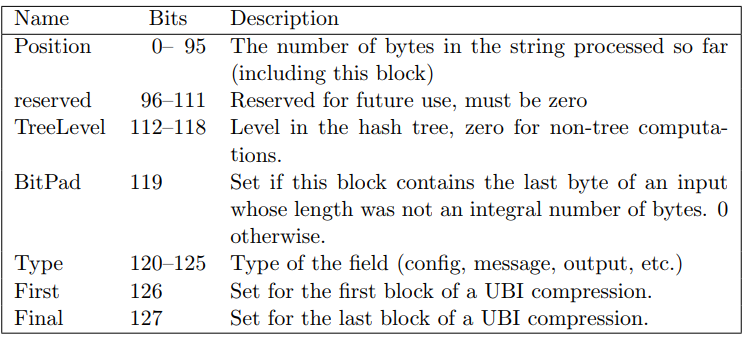
\includegraphics[width=14cm]{Images/GoldenModelDocumentation/tweak.png}
\end{center}

دلیل جمع کردن \lr{first} با ۹۶،‌ رد کردن بخش \lr{position} است. حالت اولیه \lr{first} هم به این علت با چک کردن \lr{bcount} مقداردهی شده که مقدار بخش \lr{first} باید برای سری اول گرفتن بلوک دیتا برابر با ۱ باشد. 

در این تابع ممکن است سایز دیتا دقیقا مضربی از سایز بلاک (۵۱۲) باشد،‌ برای این حالت باید مقدار بیت فیلد \lr{final} یک شود. اما این تابع از این که در حال پردازش اخرین بخش دیتا هست یا نه باخبر نیست و درنتیجه در‌ آخر ممکن است بافر شامل یک بلاک کامل از دیتا باشد. 



\subsection{\lr{skein-hash}}
\label{subsec:skein-hash}

در این تابع ابتدا هش از جنس آرایه‌ای ۶۴ تایی از کاراکتر‌های بدون علامت (\lr{uint8-t}) و سپس  \lr{ctx} ساختاری از جنس \hyperref[subsec:sph-skein-big-context]{\lr{sph-skein-big-context}} تعریف شده‌است. این هش ۵۱۲ در ۵۱۲ است و به همین دلیل حاصل نهایی هم ۶۴ بایت درنظر گرفته شده است. سپس آدرس \lr{ctx} به تابع\hyperref[subsec:sph-skein512-init]{\lr{sph-skein512-init}} پاس داده شده‌است. در این تابع مقدارهای اولیه در ‌\lr{struct} ذخیره شده‌اند. سپس تایع \hyperref[subsec:sph-skein512]{\lr{sph-skein512}} صدا شده که در آن تمام بلاک‌های دیتا به جز بلاک آخر هش و بلاک ‌اخر هم در بافر ذخیره شده‌است. سپس تابع  \hyperref[subsec:sph-skein512-close]{\lr{sph-skein512-close}} صدا شده و به آن ‌\lr{struct} و ادرس شروع \lr{hash} داده شده‌اند. در این مرحله بیت‌های اضافی اضافه شده، بلاک ‌آخر هش شده و در ‌\lr{dst} ذخیره شده‌اند. 
در نهایت ۳۲ بایت از \lr{hash} در \lr{output} ریخته شده‌است.


\subsection{\lr{sph-skein512-close}}
\label{subsec:sph-skein512-close}
\label{subsec:sph-close}
در این تابع   \hyperref[subsec:addbits]{\lr{sph-skein-addbits-and-close}}  صدا شده و به ‌آن  ساختار  \lr{cc} ،  ادرس  \lr{dst} و همین طور صفر به عنوان \lr{ub} که بیت‌های اضافه است و \lr{n} که تعداد این بیت‌های اضافه است داده شده‌اند.


\subsection{\lr{sph-skein-addbits-and-close}}
\label{subsec:addbits}
\label{subsec:sph-skein-addbits-and-close}
در این تابع  \hyperref[subsec:big-close]{\lr{skein-big-close}} با مقدار ۶۴ برای \lr{out-len} و در نهایت هم \hyperref[subsec:sph-skein512-init]{\lr{sph-skein512-init}} صدا شده‌اند. کار درهم‌سازی در \lr{skein-big-close} تمام و سپس دوباره $ h_0 $ تا $ h_7 $ از مقدارهای اولیه پر شده‌اند.


\subsection{\lr{skein-big-close}}
\label{subsec:big-close}
به این تابع ورودی‌های  \lr{sc} به عنوان ساختار هش،  \lr{ub} به عنوان بیت‌های اضافه، \lr{n} به عنوان تعداد بیت‌های اضافه،  \lr{dst} برای ذخیره هش نهایی و  \lr{out-len} به عنوان طول دیتا پاس داده شده‌اند. با توجه به هشت بیتی بودن بلوک‌ها در ابتدا حداکثر مقدار ‌\lr{n}  هشت است. در نتیجه در صورت غیر صفر بودن ‌\lr{n} ،با شیفت دادن ۱۲۸ به اندازه‌ی  \lr{n}،  متغیری به نام   \lr{z} با  \lr{n} بیت صفر در سمت راست و سپس یک بیت ۱ ساخته‌ شده‌است. سپس  با  \lr{and} کردن  \lr{ub} با    \lr{-z}،  \lr{n} بیت سمت راست  \lr{ub} صفر شده و این مقدار به \lr{x} داده شده ‌است. (زیرا  \lr{z} به صورت مکمل دو منفی شده‌است.) و سپس بیت  \lr{n+1}م  \lr{ub} با \lr{or} گرفته‌شدن با  \lr{z}  ۱ شده‌است. سپس  \hyperref[subsec:skein-big-core]{\lr{skein-big-core}} برای طول ۱ صدا شده‌است. (زیرا طول ‌\lr{x} و ماکسیموم \lr{n} یک بایت است.) و شرط بررسی   \lr{n} این‌حا به پایان رسیده‌است.
سپس \hyperref[subsec:read-state-big]{\lr{read-state-big}} صدا و بعد از ‌آن باقی‌مانده‌ی فضای بافر با ۰ پر شده‌است.
سپس دو دفعه  \hyperref[subsec:ubi-big]{\lr{UBI-BIG}}صدا شده‌است. در دفعه‌ی اول صدا شدن تابع،  \lr{etype} برابر جمع (256 + 96) با ۱۲۸ ،در صورت ۰ بودن  \lr{bcount}، و ۰ در صورت غیر صفر بودن آن قرار داده‌ شده‌است. همین‌طور در صورت غیر صفر بودن ‌ \lr{n} عدد یک هم با  \lr{etype} جمع شده‌است.  \lr{extra} هم برابر با مقدار \lr{ptr} گذاشته شده‌است،‌ که در زمان صدا کردن تابع به اخرین جایی که دیتا در بافر هست و بیت‌های بعدی ‌آن با ۰ پر شده‌اند، اشاره دارد. جمع شدن ۲۵۶ با  \lr{etype} برای یک گذاشتن  \lr{BitPad} و جمع شدن ۹۶ برای اسکیپ کردن بخش  \lr{position} است. پیش از صدا شدن تابع برای بار دوم کل بافر با ۰ پر و  \lr{bcount} هم برابر با ۰ گذاشته شده‌است. بار دوم  \lr{UBI-BIG} برای  \lr{etype} با مقدار ۵۱۲ و \lr{extra} با مقدار ۸ صدا شده‌است. در ۵۱۰ فقط بیت دوم از راست یک است، که بیت \lr{final} است و ۸ بایت بافر با ۰ پر شده‌است درنتیجه \lr{extra} هم ۸ است. 
در نهایت $ h_0 $ تا $ h_7 $ توسط \lr{sph-enc64le-aligned} بایت بایت شده و در بافر، و سپس بافر به تعداد بایت \lr{out-len} (در این‌جا ۶۴ بایت) در \lr{dst} ذخیره شده‌است.
\end{document}